\documentclass[10pt,b5paper,twoside,openright]{book}
\usepackage{config}

% From https://www.overleaf.com/learn/latex/Glossaries

\makeglossaries % Prepare for adding glossary entries


\newglossaryentry{BnB}
{
        name=B\&B,
        description={Branch and Bound}
}

\newglossaryentry{DP}
{
        name=DP,
        description={Dynamic Programming}
}

\newglossaryentry{MILP}
{
        name=MILP,
        description={Mixed Integer Linear Programming}
}

\newglossaryentry{SCIP}
{
        name=SCIP,
        description={Solving Constraint Integer Programs}
}

\newglossaryentry{MLP}
{
        name=MLP,
        description={Multi-Layer Perceptron}
}

\newglossaryentry{ML}
{
        name=ML,
        description={Machine Learning}
}

\newglossaryentry{LP}
{
        name=LP,
        description={Linear Programming}
}

\newglossaryentry{ILP}
{
        name=ILP,
        description={Integer Linear Programming}
}

\newglossaryentry{BLP}
{
        name=BLP,
        description={Binary Linear Programming}
}

\newglossaryentry{SB}
{
        name=SB,
        description={Strong Branching}
}

\newglossaryentry{GCNN}
{
        name=GCNN,
        description={Graph Convolutional Neural Networks}
}

\newglossaryentry{ReLU}
{
        name=ReLU,
        description={Recti-Linear Unit}
}

\newglossaryentry{FSB}
{
        name=FSB,
        description={Full Strong Branching}
}

\newglossaryentry{MIB}
{
        name=MIB,
        description={Most Infeasible Branching}
}

\newglossaryentry{PB}
{
        name=PB,
        description={Pseudo-cost Branching}
}

\newglossaryentry{RPB}
{
        name=RPB,
        description={Reliability Pseudo-cost Branching}
}

\newglossaryentry{NP}
{
        name=NP,
        description={Non-deterministic Polynomial-time}
}

\newglossaryentry{CPU}
{
        name=CPU,
        description={Central Processing Unit}
}

\newglossaryentry{GPU}
{
        name=GPU,
        description={Graphics Processing Unit}
}

\newglossaryentry{FiLM}
{
        name=FiLM,
        description={Feature-wise Linear Modulation}
}

\newglossaryentry{SVM}
{
        name=SVM,
        description={Support Vector Machine}
}

\newglossaryentry{COIN-OR}
{
        name=COIN-OR,
        description={Computational Infrastructure for Operations Research}
}

\newglossaryentry{MDP}
{
        name=MDP,
        description={Markov Decision Process}
}

\newglossaryentry{PO-MDP}
{
        name=PO-MDP,
        description={Partially-observable Markov Decision Process}
}

\newglossaryentry{CO}
{
        name=CO,
        description={Combinatorial Optimization}
}

\newglossaryentry{DS4DM}
{
        name=DS4DM,
        description={Canada Excellence Research Chair in Data Science for Decision Making}
}

\newglossaryentry{Ecole}
{
        name=Ecole,
        description={Extensible Combinatorial Optimization Learning Environments}
}




\addbibresource{bib/bibliography.bib}
\setlength{\cftbeforesecskip}{5pt}
\begin{document}

\pagestyle{empty}
\newcommand{\HRule}{\rule{\linewidth}{1mm}}
 
\vspace*{\stretch{1}}
\vspace*{-3.5cm}
\noindent\HRule
\begin{center}
 
\end{center}
\begin{center}
  \huge
	\large
	\noindent\emph{Engineering Cybernetics\\Master Thesis}
\end{center}
\begin{center}
 
\end{center}
\begin{center}
	\huge
	\noindent\emph{}
  \huge
  \Large
  \noindent \textbf{Ablating a Graph Neural Network for Branching in Mixed-Integer Linear Programming}
  \\ [7mm]
  \large
  \noindent\emph{Lars Lødemel Sandberg }
\end{center}
\begin{center}
  \huge
  \large
  \noindent\emph{Supervisors:\\ Prof. Lars Struen Imsland \\ Bjarne Grimstad}
\end{center}
\begin{center}
	\large
	\noindent \emph{Trondheim, 30 May 2021}
	%\noindent \emph{Trondheim, 15 June 2007}
\end{center}
\noindent\HRule
\vspace*{\stretch{2}}
\begin{figure}[h]
	\begin{center}
		\includegraphics[angle=0, width=10cm]{img/logo_ntnu}
	\end{center}
	\label{fig:logo}
\end{figure}
 
\begin{minipage}[c]{\textwidth}
	{\setlength{\baselineskip}{0.5\baselineskip}
	\small \noindent Faculty of Information Technology and Electrical Engineering\\
	\Large \noindent \textsc{department of engineering cybernetics}}
\end{minipage}

\frontmatter
\pagestyle{plain}

\begingroup
\let\cleardoublepage\clearpage
%!TEX root = ../thesis.tex
\chapter*{\englishabstractname}
\addcontentsline{toc}{chapter}{\englishabstractname}
% Multilayer Perceptrons for Learning to Branch
%
This thesis evaluates ablations of a Graph Convolutional Neural Networks for machine learning aided branching proposed by Gasse et al. (2019) \cite{gasse2019exact}
for faster solving Mixed-Integer Linear Programming (\gls{MILP}) problems. 
Efficient \gls{MILP} solution algorithms are important for real-time optimization in various industries, including industrial production, logistics, transportation, and energy production \cite{junger2010years}.  Reduced computation time via merging Machine learning with the Branch and Bound solution algorithm can improve these algorithms without sacrificing the strong benefits of global optimization.
%Multiple central researchers within mathematical programming and machine learning have recently shown interest in the application of Machine Learning in \gls{MILP} \cite{bengio2020machine,bertsimas2019online}, particularly in the variable selection part of the branching strategy \cite{khalil2020towards}.
In 2019, reliable results of improvement over top branching strategies in open-source solvers were shown \cite{gasse2019exact}, and in 2020 these methods have been expanded to purely \gls{CPU}-based solutions \cite{gupta2020hybrid}. Different network topologies and feature sets on both \gls{CPU}s and \gls{GPU}s have been presented, however, the trade-off between accuracy and efficiency with these models on varying hardware is still mostly unexplored.
In order to address this, two variants of Graph Convolutional Neural Networks and three Multi-Layer Perceptron configurations are trained via imitation learning on the Strong Branching algorithm on generated \gls{MILP} problems using the new framework \textit{Ecole} \cite{prouvost2020ecole,prouvost2021ecole}.  The models are then incorporated into the \gls{SCIP} optimization solver and evaluated on test problems. All models show near state-of-the-art efficiency when run on the \gls{GPU}. The models containing graph convolutions show a large loss of efficiency when run on the \gls{CPU} rather than the \gls{GPU}.
%Future research should attempt to implement these methods on practical optimization problems, as well as compare results to the current top proprietary solvers after parameter optimization \cite{hutter2010automated}. 

The code for this project is available at\\ \url{https://github.com/Sandbergo/branch2learn}

%
\clearpage

%!TEX root = ../Thesis.tex
\chapter*{\norwegianabstractname}
\addcontentsline{toc}{chapter}{\norwegianabstractname}
%
Denne oppgaven evaluerer ablasjoner av et grafkonvolusjonelt nevralt nettverk for maskinlæringsassistert forgrening foreslått av Gasse et al. (2019) for mer effektiv løsning av blandede heltallsproblemer (\gls{MILP}).
Effektive \gls{MILP}-løsningsalgoritmer er viktige for optimering i sanntid i mange industrier, blant annet produksjon, logistikk, transport og energiproduksjon. 
Reduksjon i beregningstid ved å kombinere maskinlæring og branch-and-bound-løsningsalgoritmen kan forbedre disse algoritmene uten å ofre de sterke fordelene til global optimering.  
I 2019 ble pålitelige resultater med forbedring over de beste forgreningsstrategiene i åpen-kildekodeløsere vist, og i 2020 ble disse metodene utvidet til rent \gls{CPU}-baserte modeller.
Forskjellige nettverkstopologier og datasett for både \gls{GPU} og \gls{CPU} har blit foreslått, men kompromisset mellom nøyaktighet og effektivitet for modellene på forskjellig maskinvare er for det meste uutforsket. 
For å adressere dette blir to grafkonvolusjonale nevralnett og tre flerlagsperceptroner trent gjennom imitasjonslæring av strong branching-algoritmen på genererte \gls{MILP}-problemer i det nye rammeverket \textit{\gls{Ecole}}. Modellene blir deretter inkorporert i optimaliseringsløseren \gls{SCIP} og evaluert på testproblemer. Alle modeller viser nær høyeste effektivitet mot sammenlignbare algoritmer på \gls{GPU}. Modellene med grafkonvolusjoner viser et mye mer betydelig effektivitetstap enn modellene uten når beregningene gjennomføres på \gls{CPU}.

Kildekoden for denne oppgaven er tilgjengelig på\\ \url{https://github.com/Sandbergo/learn2branch}
\clearpage


\tableofcontents \clearpage
\listoftables    \clearpage
\listoffigures   \clearpage
%\printglossary[type=\acronymtype] % Print acronyms
\printglossary                    % Print glossary
\endgroup


\mainmatter
\pagestyle{headings}
%!TEX root = ../Thesis.tex
\chapter{Introduction}\label{cha:introduction}
%
This chapter presents a short history, motivation and background in the fields of mathematical programming and machine learning, summarizes the previous work on the topic of \textit{learning-to-branch}, poses the research questions for the project, and explains the structure of the project.


\section{Background}

In this section, a relevant background in the relevant fields of mathematical programming and machine learning is presented, as well as an overview of the previous work in combining these fields. The section is adapted from the project report \textit{Multi-layer Perceptrons for Branching in Mixed-Integer Linear Programming }(2020). 

\subsection{Mathematical Programming}

The invention of efficient solution algorithms to linear mathematical programming problems is considered one of the great post-war inventions \cite{dantzig1983reminiscences}. The simplex algorithm and its derivatives have since become ubiquitous in a number of disciplines including finance, engineering, transportation, and energy \cite{junger2010years}. These algorithms allow for the efficient solution of the global optimum of linear functions with an objective function, a number of variables and a number of constraints on these variables. However, the simplex algorithm is limited to problems where the \textit{feasible set} of possible solutions is convex.

To further increase the expressiveness of the linear programming \textit{language}, the inclusion of non-convex constraints such as limiting variables to only take integer values, is a reoccurring limitation in modeling real-world problems in a mathematical programming language. The set of optimization problems with these integer are known as \textit{Mixed Integer Linear Programs} (\gls{MILP}). The inclusion of integer constraints to these linear problems has proved to be a very challenging problem class to develop efficient solution algorithms for, as it is considered unlikely that a polynomial-time solution algorithm exists \cite{bengio2020machine}.

For problems including integer constraints, the na\"ive approach of comparing every possible combination of feasible solutions, known as \textit{explicit enumeration}, will result in a solution algorithm that is of exponential complexity, which makes larger optimization problems intractable. An alternative to explicit enumeration is \textit{implicit enumeration}, where a large number of possible solutions so not have to be evaluated explicitly. 
\textit{Branch and Bound} (\gls{BnB}), conceived in 1960 \cite{land1960automatic}, is an algorithm for solving mathematical programming problems via implicit enumeration. It has since received numerous improvements and extensions \cite{wolsey2020integer}. 

For time-constrained applications of these non-convex optimization problems, a decrease in time to calculate the optimal solution can result in significant improvements and has been a very active field of research for many decades \cite{wolsey2020integer}. For the interested reader, the modern advances of Branch and Cut, Column Generation, and Bender's Decomposition algorithms are recommended reading in \textit{Integer Programming} by Lawrence Wolsey \cite{wolsey2020integer}.

%Currently, the most efficient solution algorithms using Branch and Bound are proprietary algorithms, notably IBM CPLEX and Gurobi, however, open source solvers do exist and are under continuous development, e.g. \gls{COIN-OR} and \gls{SCIP} Optimization Suites \cite{achterberg2009scip,anand2017comparative}. Improvements to 

There is a large interest in both theoretical and practical mathematical programming for methods that can improve the efficiency of \gls{MILP} optimization algorithms \cite{wolsey2020integer}. This can have a lasting impact on the nature of mathematical programming and is therefore an important area to explore further. Researchers in Mathematical Optimization have also noted the potential for expert-constructed branching strategies based on knowledge obtained from \textit{Statistical Learning}, also known as \textit{Machine Learning} (\Gls{ML}) \cite{lodi2017learning}.


\subsection{Machine Learning}

The current dominating paradigm of \textit{Artificial Intelligence} is \textit{Machine Learning}, where computers (algorithms) learn from experience (data) \cite{goodfellow2016deep}. The capabilities of these models have had an exponential success in recent years, much due to advances in computer hardware \cite{goodfellow2016deep}. A variety of fields have seen breakthroughs by using methods in \gls{ML}, including medical diagnostics, industrial optimization, autonomous vehicles and board games \cite{goodfellow2016deep}. 

There are a number of sub-fields within Machine Learning. In this project, the class known as \textit{supervised classification} is explored. Supervised classification is the general problem of dividing instances into classes based on past instances and their respective classes. These models learn through observing examples of past data and their classifications. The basic assumption is that the \gls{ML} model will learn from its experience, and be accurate in classifying previously unseen data. 

A prevalent field within Machine Learning the last decade is \textit{Deep Learning} (DL), where models are built up of series of nonlinear functions \cite{goodfellow2016deep}. 
The Multi-Layer Perceptron, or feedforward deep network, is the most common model in Deep Learning. Nonlinear representations are iteratively performed, giving the model a large \textit{capacity} for representing complex relations between input and output. 

For many tasks, e.g. tasks with a real-time component, the strength of Machine Learning models lies in the fast evaluation of the generated, nonlinear functions, also known as the \textit{inference} \cite{bertsimas2019online}. This strength makes it possible for machines to take over tasks previously thought to require a human operator, or increase efficiency greatly via automation.

Further, the results of the iterative optimization process of generating an \gls{ML}-model can find patterns in data that are difficult to discover with traditional statistics \cite{goodfellow2016deep}. Much like chess Grandmasters learn from observing the best AI-players, so too might experts gain knowledge in their respective fields by analyzing the results of an algorithm built on statistical learning.  


\section{Previous Work}

There has been a recent surge of interest in leveraging machine learning methods in solving non-convex optimization problems, notably a recent literature review conducted by Yoshua Bengio \cite{bengio2020machine}. The aim is for statistical learning to aid in the efficient solving of complex problems without sacrificing the strong guarantees inherent in mathematical optimization solvers. These hybrid methods now show the potential to be competitive with the state-of-the-art solvers for these \gls{NP}-hard problems \cite{gasse2019exact}. 

An overview of the history of learning in \gls{BnB} is given a survey paper by Lodi and Zarpellon \cite{lodi2017learning}. To summarize, interest in using more advanced statistics to unravel the relations of a \gls{MILP} problem and the optimal branching variable was first observed in 2009. Various approaches to learning have been attempted, with recent efforts to directly incorporate the learned algorithms into the solution algorithm from 2016 and onwards \cite{lodi2017learning}.  

A thorough look into the possibilities of machine learning in \gls{BnB} was conducted by Elias Khalil \cite{khalil2020towards}, in which he chose the term \textit{data-driven algorithm design} for this approach. 
In \textit{Learning to Branch} (2016) \cite{khalil2016learning} imitation learning of Strong Branching was performed as a learn-to-rank-problem. The algorithm was competitive with a selection of modern solvers \cite{khalil2016learning}. 
Recent advances using\textit{ Graph Convolutional Neural Networks} (\Gls{GCNN}) have proved to consistently improve on the solution time of the best available open-source solvers by Gasse et al.  \cite{gasse2019exact}. 

The promising results found by Gasse et al. \cite{gasse2019exact} were, however, criticized by Gupta et al. \cite{gupta2020hybrid} for reliance on modern \gls{GPU} processing power. They showed that the efficiency of the GCNN-aided algorithm did not improve on the native branching strategies when run on a CPU. Gupta et al. presented novel methods running only on the CPU that were able to improve significantly on the native strategies. These methods include \textit{Support Vector Machines} (\Gls{SVM}), \textit{Multi-Layer Perceptrons} (\Gls{MLP}) and  \textit{Feature-wise Linear Modulation Models} (\gls{FiLM}) \cite{gupta2020hybrid}. 

Though GPU-aided algorithms are interesting in their own right, a fair comparison of algorithmic efficiency cannot be made when the machine learning-based models are aided by expensive, advanced and specialized GPU processing power, as in Gasse et al. \cite{gasse2019exact}. 
For this reason, all analysis of computational efficiency in this project will be performed on a CPU. Nevertheless, discrete optimization performed on GPUs is a very interesting topic, for a discussion on Branch and Bound algorithms on GPUs the reader is referred to Schultz et al. \cite{schulz2013gpu}. It is also assumed by the author that advances in ML-aided optimization can combine nicely with advances in parallel computing.

The methods of Gasse et al. \cite{gasse2019exact} and the improvements made by Gupta et al. \cite{gupta2020hybrid} have shown that data-driven methods can improve upon existing state-of-the-art solvers, and is therefore an avenue worth examining, exploring, and expanding further. Machine Learning is a rapidly developing field, and recent advances have shown to outclass the early proof-of-concept attempts, sometimes by considerable margins \cite{holzinger2018current}. There is little reason to believe that ML-leveraged algorithms do not have this latent potential. 

Recent attempts to facilitate the development of \gls{ML}-aided \gls{CO} includes a notable project named Extensible Combinatorial Optimization Learning Environments (\emph{Ecole}) \cite{prouvost2020ecole}. It was developed by the group Data Science For Decision Making (\gls{DS4DM}), connected to the Polytechnique Montr\'{e}al university. \gls{Ecole} is an open source framework for a controllable python interface to \gls{BnB} algorithms, and is built on SCIP and PySCIPOpt. The framework is tightly knit with the previous work from the group, notably Gasse et al. \cite{gasse2019exact} and Gupta et al. \cite{gupta2020hybrid}, and aims to standardize research within the field of \gls{BnB} algorithm improvement.  
As of May 2021, no articles have been published with results from using this framework. A recent article by
Cappart et al. (2021) \cite{cappart2021combinatorial} presents the current status of and the role of the \gls{Ecole} framework in further developing this field. 


\section{Research Questions}\label{sec:questions}

For this project, three research questions are considered.
%
\begin{enumerate}[label=(\roman*)]
    \item \textit{Can Graph Convolutional Neural Networks and  Multi-Layer Perceptrons decrease the running time of Branch and Bound running on the \Gls{CPU}?}
\end{enumerate}
%
A Multi-Layer Perceptron model is implemented by Gupta et al. \cite{gupta2020hybrid}, however it is used in the context of hybrid models, combining \Gls{GCNN} features with the general variable features. This is done to mitigate the loss in efficiency by running \gls{GCNN}s on the \gls{CPU}. It is unclear whether a purely \gls{MLP}-based approach can result in improvements on the native branching strategies. \gls{MLP}s have been the focus of research for many decades, and implementation is assumed to be relatively straightforward \cite{goodfellow2016deep}.
%
\begin{enumerate}[resume*]
    \item \textit{What is the impact of different \gls{GCNN} and \gls{MLP} model topologies on the accuracy and efficiency of the Branch and Bound algorithm, when run on the \gls{CPU} and \gls{GPU}}?
\end{enumerate}
%
Machine Learning model choice based on reduced complexity is cited as a motivation for design choices in Gupta et al. \cite{gupta2020hybrid}, however the impact of varying sizes of the same model has not been performed before, and the magnitude of the impact is unknown. Increased model capacity is known to facilitate higher accuracy \cite{goodfellow2016deep}, however, whether this has a detrimental effect on the Branch and Bound algorithm's overall performance is unknown. Results from methods that are more comparable will indicate the importance of accuracy versus computational complexity.   
%
\begin{enumerate}[resume*]
    \item \textit{What are the most promising research opportunities for learning in Branch and Bound?}
\end{enumerate}
%
The general field has gained traction recently \cite{bengio2020machine}, and the author assumes more research and interest will come in the next few years. In the implementation of this project, the new framework \gls{Ecole} is used. This is the first paper where \gls{Ecole} is used as the basis for the experiments, and an independent review of this framework is due.  



\section{Thesis Structure}

In the following chapter, \Cref{cha:background}, the necessary theoretical background in optimization and machine learning is presented, as well as a review of earlier work in the field. In \Cref{cha:methods}, the data set, chosen training and testing methods, and experiments are presented, along with the architectural choices. \Cref{cha:results} provides the results of the aforementioned experiments. Then, \Cref{cha:discussion} contains discussions of the results, a critique of the experiments, and ideas for further work. Finally, \Cref{cha:conclusion} summarizes the project with a conclusion on the implications of the results. 



\chapter{Background}\label{cha:background}

The following chapter lays the theoretical groundwork for the project. An understanding of linear algebra, numerical optimization, algorithms, and statistics is assumed. 

\section{Mathematical Programming}

In this project, the terms mathematical programming, numerical optimization, and optimization are used interchangeably.


\subsection{Linear Programming}

In mathematical programming, the general linear problem can be stated as \cite{gasse2019exact}:
\begin{align} \label{eq:lp}
    \underset{\mathbf{x}}{\arg \min }\left\{\mathbf{c}^{\top} \mathbf{x} \; \mid \mathbf{A} \mathbf{x} \leq \mathbf{b},\; \mathbf{x} \in \mathbb{R}_+^{n}\right\},
\end{align}
where $ \mathbf{x} \in \mathbb{R}_+^n$ is the variable vector
with the objective coefficient vector $c \in R^n $, 
the constraint coefficient matrix $\mathbf{A} \in R^{m \times n}$
and the constraint right-hand-side vector $b \in R^m $.

The size of the problem will be measured by the dimensions of the constraint coefficient matrix $ \mathbb{A} $, where the number of rows and columns corresponds to the number of variables and constraints, respectively.

These problems are convex \cite{wolsey2020integer}, and can be solved by several efficient algorithms. The simplex algorithm can solve problems on this form efficiently, as optimal points are guaranteed to be on the vertices of the feasible set, and the same for interior-point methods \cite{nocedal2006numerical}. These algorithms are good average performance but do not have guaranteed polynomial running time in the worst case. Guaranteed polynomial solution algorithms do exist, for instance Karamkar's algorithm \cite{karamkar1984new}. 


\subsection{Mixed Integer Linear Programming}

Mixed Integer Linear Programming is a superset of linear programming, where one or more of the variables can be restricted to discrete values. The general problem can in this case be stated as \cite{gasse2019exact}:
\begin{align}\label{eq:milp}
    \underset{\mathbf{x}}{\arg \min }\left\{\mathbf{c}^{\top} \mathbf{x} \mid \mathbf{A} \mathbf{x} \leq \mathbf{b}, \; \mathbf{x} \in \mathbb{Z}_+^{p} \times \mathbb{R}_+^{n-p}\right\},
\end{align}
where $ p $ is the number of integer variables, otherwise the variables are the same as \Cref{eq:lp}.

% https://texample.net/tikz/examples/colored-diagram/
\begin{figure}
    \centering
    \begin{tikzpicture}[
        thick,scale=0.5, 
        every node/.style={scale=0.2}
        every path/.style = {},
        every node/.append style = {font=\sffamily}
      ]
      \begin{scope}
        \shade[right color=gray, left color=white, opacity=0.7]
          (-0.5,-0.5) rectangle (0,6.5);
        \node[rotate=90, above] at (0,3) {};
        \shade[top color=gray, bottom color=white, opacity=0.7]
          (-0.5,-0.5) rectangle (8.5,0);
        \shade[left color=gray, bottom color=gray, right color=white, opacity=0.5]
          (-0.5,5.5) -- (8.5,3) -- (8.5,6.5) -- (-0.5,6.5) -- cycle;
        \path (-0.5,5.5) -- node[pos=0.23, sloped, above] {}
          (8.5,3);
        \shade[left color=gray, right color=white, opacity=0.5]
          (2.5,6.5) -- (8.5,6.5) -- (8.5,0) -- (5,0) -- cycle;
        \path (5,0) -- node[pos=0.3, sloped, above] {} (2.5,6.5);
        \node[text width=6em, align=center] at (2,2)
          {};
        \draw[->] (-0.5,0) -- (8.5,0) node[below] {x};
        \draw[->] (0,-0.5) -- (0,6.5) node[above] {y};
        \node[rotate=-45, above, text width=9em, align=center] at (7.25,5.25)
          {};
        \path[clip] (-0.5,-0.5) rectangle (8.5,6.5);
        \foreach \i in {0.5,3,...,13} {
          \draw[help lines] (-0.5,\i) -- +(-45:15);
        }
      \end{scope}
      \draw[very thick, ->] (9,3.25) -- node[above, text width=3cm, align=center]
        {} (11.5,3.25);
      \begin{scope}[shift={(13,0)}]
        \shade[right color=gray, left color=white, opacity=0.7]
          (-0.5,-0.5) rectangle (0,6.5);
        \shade[top color=gray, bottom color=white, opacity=0.7]
          (-0.5,-0.5) rectangle (8.5,0);
        \shade[left color=gray, bottom color=gray, right color=white, opacity=0.5]
          (-0.5,5.5) -- (8.5,3) -- (8.5,6.5) -- (-0.5,6.5) -- cycle;
       \shade[left color=gray, right color=gray, opacity=0.5]
         (2.5,6.5) -- (8.5,6.5) -- (8.5,0) -- (5,0) -- cycle;
        \draw[->] (-0.5,0) -- (8.5,0) node[below] {x};
        \draw[->] (0,-0.5) -- (0,6.5) node[above] {y};
        \foreach \i in {0,1,...,6.5} {
          \draw[help lines] (-0.5,\i) -- (8.5,\i);
        }
        \foreach \i in {2,4,...,8.5} {
          \draw[help lines] (\i,6.5) -- (\i,-0.5);
        }
        \foreach \i in {0,1,...,5} {
          \node[draw,cross out,label={left:\i}] at (0,\i) {};
        }
        \foreach \i in {0,1,...,4} {
          \node[draw,cross out] at (2,\i) {};
        }
        \foreach \i in {0,1,...,2} {
                \node[draw,cross out] at (4,\i) {};
        }
        \foreach \i in {0,2,...,6} {
          \node[below] at (\i,0) {\pgfmathparse{int(\i/2)}\pgfmathresult};
        }
      \end{scope}
    \end{tikzpicture}
    \caption{Figure of an \Gls{LP} and the corresponding \Gls{ILP}}
    \label{fig:milpfig}
\end{figure}

In \Cref{fig:milpfig}, an \gls{LP} problem and the problem with integrality constraints is shown. For the LP problem, the shaded areas represent the inequality constraints, where the diagonal lines represent the level curves of the objective function. In the \gls{ILP} problem, the crosses represent the feasible solutions. The LP is also called a \textit{relaxation} of the original \gls{ILP}, which is fundamental to efficient solving algorithms of \gls{MILP} problems.

A problem that includes integrality constraints cannot be convex \cite{wolsey2020integer}. The non-convexity of the feasible set of the problem constitutes a significant challenge, and it is considered unlikely that polynomial-time solutions exist \cite{papadimitriou1982combinatorial}. \gls{MILP} problems belong to the category of \gls{NP}-hard problems \cite{papadimitriou1982combinatorial}.   



A subset of \gls{MILP} problems can be Integer Linear Programming (\gls{ILP}), where all variables are restricted to integer values, or Binary Linear Programming (\gls{BLP}), where all variables are restricted to binary values. 

\gls{ILP} and \gls{BLP} problems belong to the category of combinatorial optimization problems, which has been the main focus of the efforts to solve entirely or partially with machine learning methods \cite{bengio2020machine}. 


\section{Branch and Bound}\label{sec:bnb}

A \textit{relaxation} of a \gls{MILP} problem is achieved by relaxing the integrality constraint, as shown in \Cref{fig:milpfig}. Obtaining the solution to the relaxed problem gives a lower bound on the optimal solution (for a minimization problem). Naturally, any feasible solution to the integrality-constrained problem gives an upper bound on the solution. Furthermore, if the solution to the relaxed problem adheres to the integrality constraints, it is also the solution to the MILP problem \cite{wolsey2020integer}.

The most prevalent solution algorithm for MILP problems exploits these results, by sequentially dividing the solution space until the optimum with the integrality constraint is found. This is done by branching in a bipartite graph according to \cite{gasse2019exact}:
\begin{align} \label{eq:branch}
    x_{i} \leq\left\lfloor x_{i}^{\star}\right\rfloor \vee x_{i} \geq\left\lceil x_{i}^{\star}\right\rceil, \quad \exists \; i \leq p \mid x_{i}^{\star} \notin \mathbb{Z}    
\end{align}
Further creating sub-problems with this binary decomposition. An illustration of this process is shown in \Cref{fig:bandb1}.

%https://tex.stackexchange.com/questions/416359/branch-and-bound-tree-in-tikz
\comments{
\begin{figure}
\centering
\begin{forest}
  branch and bound,
  where level=1{
    set branch labels={x\leq}{}{x\geq}{},
  }{
    if level=2{
      set branch labels={}{\geq y}{}{\leq y},
    }{},
  }
  [1055.56:S:950
    [1000:S_1:950:5
    ]
    [1033:S_2:950:6
      [1033:{S_2,1}:950:1]
      [950:{S_2,2}:1033:2]
    ]
  ]
\end{forest}
\caption{\label{fig:bandb1}PLACEHOLDER Illustration of the branch and bound algorithm}
\end{figure}}

\begin{figure}
\centering
\includegraphics[width=0.8\linewidth]{img/bnb.png}
\caption{\label{fig:bandb1}Illustration of the branch and bound algorithm adapted from a maximization problem in \textit{Integer Programming }(2020) \cite{wolsey2020integer}}
\end{figure}

For each generated solution, represented by nodes in \Cref{fig:bandb1}, a relaxation of the problem is solved in order to obtain an upper and lower bound on the solution of the sub-problem. 
These values are shown on the top and bottom right, respectively. 
Generating upper and lower bounds for solutions allow for discarding a large number of solutions \cite{wolsey2020integer}. Branches can be \textit{pruned} (meaning no further partitioning from that branch) if they meet at least one of the following three criteria \cite{wolsey2020integer}:
\newpage
\begin{enumerate}[label=(\roman*)]
    \item Pruning by optimality: $Z^t = \{\max \bm{c}^{\top} \bm{x} : \bm{x} \in S_t\}$ has been solved.
    \item Pruning by bound: $\overline{Z}^t \leq \underline{Z}^t$.
    \item Pruning by infeasiblity: $S_t = \emptyset $.
\end{enumerate}
For \Cref{fig:bandb1}, the graph on the right represents the tree after solving the relaxation, resulting in $S_2$ being pruned by infeasibility, $S_3$ cut off by bound and $S_4$ pruned by optimality.


The choice of node and variable to branch on to find the optimum in the fewest number of branching processes is central to an efficient implementation of \gls{BnB}. Partitioning the feasible set such that the node with the optimal value (criteria i) is found in the fewest possible branchings is the optimal strategy. 


\subsection{Valid Inequalities}\label{ssec:inequalities}

Another important method used in \gls{BnB} algorithms is the concept of valid inequalities. A valid inequality is an inequality that does not remove feasible solutions of the non-convex solution set but can remove potential solutions to the relaxed problems. A valid inequality can be expressed as:
\begin{equation}\label{eq:cut}
    \bm{\pi}^{\top} \bm{x} \leq \pi_0 \quad \forall \; \mathbf{x} \in  \bm{X}   
\end{equation}
where $\bm{X}$ is the feasible set as described in \Cref{eq:milp}. These inequalities reduce the size of the feasible set for the relaxations of the problem without removing feasible solutions of the original problem. An illustration of an \gls{ILP} with an added valid inequality is shown in \Cref{fig:cut}. Here the feasible set of the relaxation is reduced in size by the added constraint, while the feasible points of the \gls{ILP} remain feasible after the application of the inequality, as is given in \Cref{eq:cut}.

\begin{figure}
    \centering
    \begin{tikzpicture}[
        thick,scale=0.5, 
        every node/.style={scale=0.2}
        every path/.style = {},
        every node/.append style = {font=\sffamily}
      ]
      \begin{scope}
        \shade[right color=gray, left color=white, opacity=0.7]
          (-0.5,-0.5) rectangle (0,6.5);
        \shade[top color=gray, bottom color=white, opacity=0.7]
          (-0.5,-0.5) rectangle (8.5,0);
        \shade[left color=gray, bottom color=gray, right color=white, opacity=0.5]
          (-0.5,5.5) -- (8.5,3) -- (8.5,6.5) -- (-0.5,6.5) -- cycle;
       \shade[left color=gray, right color=gray, opacity=0.5]
         (2.5,6.5) -- (8.5,6.5) -- (8.5,0) -- (5,0) -- cycle;
        \draw[->] (-0.5,0) -- (8.5,0) node[below] {x};
        \draw[->] (0,-0.5) -- (0,6.5) node[above] {y};
        \foreach \i in {0,1,...,6.5} {
          \draw[help lines] (-0.5,\i) -- (8.5,\i);
        }
        \foreach \i in {2,4,...,8.5} {
          \draw[help lines] (\i,6.5) -- (\i,-0.5);
        }
        \foreach \i in {0,1,...,5} {
          \node[draw,cross out] at (0,\i) {};
        }
        \foreach \i in {0,1,...,4} {
          \node[draw,cross out] at (2,\i) {};
        }
        \foreach \i in {0,1,...,2} {
                \node[draw,cross out] at (4,\i) {};
        }
      \end{scope}
      \draw[very thick, ->] (9,3.25) -- node[above, text width=3cm, align=center]
        {} (11.5,3.25);
      \begin{scope}[shift={(13,0)}]
        \shade[right color=gray, left color=white, opacity=0.7]
          (-0.5,-0.5) rectangle (0,6.5);
        \shade[top color=gray, bottom color=white, opacity=0.7]
          (-0.5,-0.5) rectangle (8.5,0);
        \shade[left color=gray, bottom color=gray, right color=white, opacity=0.5]
          (-0.5,5.5) -- (8.5,3) -- (8.5,6.5) -- (-0.5,6.5) -- cycle;
        \shade[left color=gray, right color=gray, opacity=0.5]
          (2.5,6.5) -- (8.5,6.5) -- (8.5,0) -- (5,0) -- cycle;
        \shade[left color=gray, right color=gray, opacity=0.5]
          (0.0,6.5) -- (8.5,6.5) -- (8.5,0) -- (6.0,0) -- cycle;
        \draw[->] (-0.5,0) -- (8.5,0) node[below] {x};
        \draw[->] (0,-0.5) -- (0,6.5) node[above] {y};
        \foreach \i in {0,1,...,6.5} {
          \draw[help lines] (-0.5,\i) -- (8.5,\i);
        }
        \foreach \i in {2,4,...,8.5} {
          \draw[help lines] (\i,6.5) -- (\i,-0.5);
        }
        \foreach \i in {0,1,...,5} {
          \node[draw,cross out] at (0,\i) {};
        }
        \foreach \i in {0,1,...,4} {
          \node[draw,cross out] at (2,\i) {};
        }
        \foreach \i in {0,1,...,2} {
                \node[draw,cross out] at (4,\i) {};
        }
      \end{scope}
    \end{tikzpicture}
    \caption{Figure of \Gls{ILP} before and after an added valid inequality.}
    \label{fig:cut}
\end{figure}
 


Algorithms that find these inequalities during the \gls{BnB} algorithm are called \textit{Branch and Cut}. The nomenclature comes from calling the application of these inequalities \textit{cuts} or \textit{cutting planes}.
When an application of inequalities are only employed on the root node (before dividing the solution space in the enumeration), the algorithm is sometimes referred to as \textit{Cut and Branch} rather than \textit{Branch and Cut} \cite{wolsey2020integer}.


\subsection{Branching Variable Selection Strategy}\label{ssec:branchingstrategy}

As mentioned, an important decision in the B\&B algorithm is the choice of the variable that should be branched on. 
There exists many heuristics for solving this, which vary in computational complexity and accuracy. 
A good branching algorithm should choose to branch on variables that lead to small solution trees (fewer nodes evaluated) and find these variables in a computationally efficient manner. 

The current branching strategy resulting in the smallest solution trees is known as \textit{Strong Branching} (\gls{SB}) \cite{applegate1995finding}, and the application of this branching strategy at every node is known as \textit{Full Strong Branching} (\gls{FSB}) \cite{achterberg2004branching}. 
This branching policy is based on determining the best variable to branch on by solving the relaxation for every candidate variable and is therefore very computationally expensive compared to other methods \cite{achterberg2004branching}.

All popular variable selection strategies depend on scoring all the possible variables and selecting the variable with the most optimal score \cite{achterberg2004branching}. There are two other classes of branching strategies than \gls{FSB}: \textit{Most Infeasible Branching} (\gls{MIB}), where the variable with the fractional part of the relaxation optimum closest to $0.5$ is selected (a very poor strategy) 
and \textit{Pseudo-cost Branching} (\gls{PB}), which relies on the expected change in objective value based on previous branching on the variable in question
\cite{achterberg2004branching}. Today, combinations of \gls{FSB} and \gls{PB} are most common \cite{anand2017comparative}.   

In the literature, the branching strategy is referred to as a strategy, policy, or rule, in this project \textit{strategy} is used.  


\section{Learned Branching Policy}

Recently, attempts have been made to find a branching strategy based on statistical learning. 

Using machine learning, specifically imitation learning, to find good candidate variables for branching in a less computationally demanding manner was proposed by Elias Khalil \cite{khalil2016learning}. Various methods for learning in branching include \textit{ Support Vector Machine Ranking} (\Gls{SVM}) \cite{khalil2016learning}, \textit{Graph Convolutional Neural Networks} (\gls{GCNN}) \cite{gasse2019exact} and \textit{Feature-wise Linear Modulation} (\gls{FiLM}) \cite{gupta2020hybrid}.

The fundamental assumption to this approach is that the most computationally demanding but most accurate branching policy can be learned. The algorithm will use imitation learning on the branching expert to find a computationally less expensive non-linear function approximation to the expert algorithm's variable scoring. Then, the algorithm branches on the variable with the highest score. This can be expressed as: 
\begin{align}
    f(i) &=  \pi_{SB} (i) + \epsilon \quad \forall \; i \in \mathcal{C}\\
    f(i) &= s_i\\
    i^*_f &= \underset{i \in \mathcal{C}}{\mathrm{argmin}} \; \bm{s}_i
\end{align}
where $f$ is the learned function, $\mathcal{C}$ is the set of possible branching variables, $\pi_{SB}$ is the Strong Branching strategy and $\epsilon$ is the deviation in the scoring function. 


\section{Multi-layer Perceptrons}

Multi-Layer Perceptrons (MLP), more commonly known as deep feed-forward neural networks, are recommended by Gupta et al. (2020) \cite{gupta2020hybrid} as a less computationally expensive alternative to the approaches by Khalil et al. (2016) \cite{khalil2016learning} and Gasse et al. (2019) \cite{gasse2019exact}. 

MLPs are networks that generate a nonlinear function $y = f(\mathbf{x}; \bm{\theta})$, where $x$ is the input $y$ is the output and $\bm{\theta}$ represents the parameters of the function. The parameters are learned during repeated optimization, and will under ideal circumstances converge to approach the goal function $y = f^*(\mathbf{x})$. The function is realized as a series of compositions of functions. The composed functions are represented as an acyclical, directed graph \cite{nielsen2018neural}, and can be expressed as:
\begin{align}
    y = f_L \circ f_{L-1} \circ \ldots \circ f_{1} \circ f_{0} (\mathbf{x})  
\end{align}
The functions are denoted as layers of the perceptron, and are implemented as affine functions of every input parameter at every node, $\mathbf{z}_l = \mathbf{x}_{l-1}^T \mathbf{w}_l + \mathbf{b}_l$. Applying non-linear function, known as an \textit{activation function}, allows the \gls{MLP} to represent arbitrary nonlinear functions \cite{goodfellow2016deep}. This is expressed as $\mathbf{x}_l = \mathbf{a}(\mathbf{z}_l)$.

The computation of the output of the function given its input is known as a \textit{forward pass} through the network. The required computations for a single input vector into a network with $ n $ hidden layers will include $ n + 1 $ matrix multiplications and $ n + 1 $ applications of the non-linear activation function, given that there is an activation function on the output. 

Depending on the training configuration, the problem can be interpreted as a classification problem or regression problem (or a ranking problem, as in \cite{khalil2016learning}). In the following experiments, the former approach is selected, as has become popular after Gasse et al. (2019) \cite{gasse2019exact}. 





\section{Markov Decision Processes}\label{sec:mdp}

Central to the advancement of learned strategies in \gls{BnB} is the interpretation of the solution algorithm as a \textit{Markov Decision Process} (\gls{MDP}) \cite{gasse2019exact}. This interpretation relates the problem to a large collection of literature on the topic \cite{howard1960dynamic}.

An \gls{MDP} is expressed as $ \mathcal{S}, \mathcal{A}, p_{init}, p_{trans}, R$ 
where $ \mathcal{S}$ is the state space, 
$\mathcal{A}$ is the action space, 
$p_{init}$ is an initial state distribution ($p_{init}\;:\;\mathcal{S}\leftarrow \mathbb{R}_{\geq 0}$), 
$p_{trans}$ is the state transition distribution (
$p_{trans}\; : \; \mathcal{S}
\times \mathcal{A}\times \mathcal{S}
\leftarrow \mathbb{R}_{\geq 0}$), 
$p_{trans}$), $R$ is the reward function $R\;:\;\mathcal{S} \rightarrow \mathbb{R}$. \cite{prouvost2020ecole}. 

Further, the \textit{action policy} $\pi$ is given as $\pi \; : \; \mathcal{A}\times \mathcal{S}
\leftarrow \mathbb{R}_{\geq 0}$, and results in state-action trajectories $\tau = (s_0, a_0, s_1, a_1, ... )$ that obey a joint distribution that can be expressed as following: \cite{prouvost2020ecole}
\begin{equation}
    \tau \sim \underbrace{p_\textit{init}(s_0)}_{\text{initial state}}
\prod_{t=0}^\infty \underbrace{\pi(a_t | s_t)}_{\text{next action}}
\underbrace{p_\textit{trans}(s_{t+1} | a_t, s_t)}_{\text{next state}}
\end{equation}

These definitions now allow a formulation of the \gls{MDP} control problem, which is the problem of interest in this thesis. The control problem consists of finding the action policy that maximizes the reward, and can be stated as: \cite{prouvost2020ecole}
\begin{equation}\label{eq:mdprcontrol}
    [\pi^\star = \underset{\pi}{\operatorname{arg\,max}}
\lim_{T \to \infty} \mathbb{E}_\tau\left[\sum_{t=0}^{T} R(s_t)\right]
\end{equation}


\subsection{Partially-observable Markov Decision Processes}

A subset or generalization of an \gls{MDP} is the \textit{Partially-observable Markov Decision Process }(\gls{PO-MDP}) \cite{monahan1982state}. Processes of this class allows for uncertainty of the states as well as additional acquisition of state information \cite{monahan1982state}.
The addition of an observation of the process in the observation space ($o \in \Omega $) extends the process to the formulation to $ (\mathcal{S}, \mathcal{A}, p_{init}, p_{trans}, R, O)$. 

The generalization from \gls{MDP} to \gls{PO-MDP} concedes the Markovian nature of the trajectories \cite{prouvost2020ecole}, i.e:
\begin{equation}
    o_{t+1},r_{t+1} \not \perp   h_{t-1} \mid o_t,r_t,a_t
\text{,}
\end{equation}
meaning that the entire action-state history of the process is necessary for the policy. The history is denoted $\mathcal{H}$, and the policy of the \gls{PO-MDP} is stated as:
\begin{equation}
    \pi:\mathcal{A} \times \mathcal{H} \to \mathbb{R}_{\geq 0}
\end{equation}
which means that the control problem of the \gls{PO-MDP} can also be stated as \cref{eq:mdprcontrol}.

\subsection{Branch \& Bound as a \gls{PO-MDP}}

Interpreted in the language of \gls{MDP}s, the \gls{BnB} algorithm is the \textit{environment} and a concrete \gls{MILP} problem instance is an \textit{episode} in this environment. The \textit{agent} is the brancher, where in this thesis the variable selection policy is the component of interest, ignoring the node selection policy. The state of the solver consists of the \gls{BnB} tree at that instance, as well as the observations at each node (the \textit{history} of the \gls{PO-MDP}).

This formulation is the basis for the \textit{Ecole} framework, which is discussed in \Cref{sec:ecole}
The \gls{PO-MDP} formulation allows for the agent in the \gls{BnB} environment to be learned through \textit{reinforcement learning}


\section{Reinforcement Learning}

The subset of machine learning described as Reinforcement Learning (\gls{RL}) is highly relevant in the context of \gls{ML} in \gls{CO}. 

Many attempts have been made at implementing \gls{RL} in \gls{CO}, see for example ... Attempts show promise, however the approaches rely on efficient and accurate models pre-trained on labeled data. 
\footnote{Attempts on \gls{RL} models were also made by the author of this thesis, but the models did not prove useful with the chosen method.}
Cappart et al. (2021) \cite{cappart2021combinatorial} also conclude that useful \gls{RL} policies are not mature yet. 


\section{Graph Convolutional Neural Networks }

Graph Convolutional Neural Networks (\gls{GCNN}s) is a term for neural networks that have input data represented in a graph-structure that is processed by the convolution operation \cite{kipf2016semisupervised}. The graph convolution operation is defied by the propagation rule \cite{kipf2016semisupervised}:
\begin{equation}
    H^{(l+1)} = \sigma \left( \Tilde{D}^{-\frac{1}{2}} \Tilde{A} \Tilde{D}^{-\frac{1}{2}} H^{(l)}W^{(l)}\right)
\end{equation}
where $H^{(l)}$ is the matrix of activations in layer $l$ (meaning $H^{(0)} = 0$). $\Tilde{A} = A + I_N$, where $A$ is the adjacency matrix representing the undirected graph $\mathcal{G}$, and $\Tilde{D} = \sum_j \Tilde{A}_{i j}$. $\sigma( \cdot) $ is a nonlinear activation function.
This operation is shown to be inspired by the first order approximations to spectral filters on graphs \cite{kipf2016semisupervised}.

The term \textit{embeddings} will be used in this thesis for continuous-variable representations derived from the input features, as it is used in Gasse et al. \cite{gasse2019exact}. 

Models that leverage the graph nature of combinatorial optimization problems have been shown to have satisfactory performance, see e.g. Dai et al. (2018) \cite{dai2018learning}. 
\gls{GCNN}s are proposed by Gasse et al. \cite{gasse2019exact} as an alternative to the feature-rich approaches by Khalil et al. (2016) \cite{khalil2016learning}. 
The application of \gls{GCNN}s on \gls{BnB} algorithms relies on the bipartite graph structure that results from the solution process, as explained in \Cref{sec:bnb}. At each point before the variable selection process, the state of the solution algorithm graph can be processed by the \gls{GCNN} algorithm. 

The state of the \gls{BnB} graph at a node can be represented as $s_t = (\mathcal{G}, \mathbf{C}, \mathbf{E}, \mathbf{V})$, where $\mathcal{G}$ represents the bipartite \gls{BnB} solution graph at that time instance, $\mathbf{C}$ represents the constraints, $\mathbf{E}$ represents the \textit{edges}, or connections between the variables and constraints, and $\mathbf{V}$ represents candidate variables.  
\chapter{Methods}\label{cha:methods}

In this chapter, the selected methods for the experiments are presented and discussed.  
An understanding of the theoretical groundwork of the project from \Cref{cha:background} is assumed. Most methods are taken directly or indirectly from the source code of Gasse et al. \cite{gasse2019exact} and Gupta et al. \cite{gupta2020hybrid}, except for the choice of \gls{MLP} configurations.


\section{Dataset}\label{sec:dataset}

This section presents the selected data set and the process of generating trainable and testable data for the perceptrons. 


\subsection{Problem Instances}\label{ssec:probleminstances}

In order to evaluate the methods presented in this project to the previous advances in the field, artificially generated \gls{MILP} problems found in Gasse et al. \cite{gasse2019exact} are used to train and evaluate the models. These problems are also the standard implemented in \gls{Ecole}.
The problems are expressed as pure binary programs. The results of the algorithm are, however, generalizable to general \gls{MILP} problems, as it extends the general \gls{BnB} algorithm \cite{gasse2019exact}. 

Problems are generated in three sizes: small, medium, and large. Small instances are used for training, while medium and large problem sizes are reserved for evaluating the extended algorithm's ability to generalize on more challenging problems. These problem sizes represent what current algorithms can solve within seconds (for the small instances) and multiple minutes (for the large instances).


\subsubsection{Set Covering}

The set covering problem is implemented in \gls{Ecole} as described in Balas \& Ho (1980)\cite{balas1980set} \footnote{The available version of this paper contains nearly illegible equations, the article Minoux (1987) \cite{minoux1987class} has therefore been used to supplement.}. The general problem includes a set of vertices $V_j$ and a matrix of costs $c_j$ for activating an edge between any two vertices. The activation of an edge is modelled with the binary variable $x_j$ and the characteristic vector of subset $V_j$ denoted $\textbf{A}_j$. The binary linear problem of covering all vertices at minimum cost can be expressed as: 
\begin{align}
    \min &\sum_{j=1}^N c_j x_j \\ s.t. \; &\sum_{j=1}^N \mathbf{A}_j x_j \geq \mathbf{1} \,,\; x \in \mathbb{B}^N 
\end{align}
The problem is therefore a pure binary linear problem with only inequality constraints. The set covering problem is a well-known class, and is one of Karp's 21 \gls{NP}-complete problems \cite{karp1972reducibility}.  

\subsubsection{Combinatorial Auction}

The combinatorial auctions problem was chosen out of the four because it has consistently proved to be the most challenging of the four problems \cite{gasse2019exact} \cite{gupta2020hybrid}. The problem is implemented by Gasse et al. \cite{gasse2019exact}, and is based on the formulation presented in Leyton-Brown et al. \cite{brown2000towards}.  

The combinatorial auctions problem is based on multi-object auctions where bidders place monetary bids on bundles (combinations) of goods, and the optimization problem is to find the bids that maximize the profit of the auctioneer \cite{brown2000towards}. The problems are considered realistic and economically oriented, and are applicable to five broad domains in which optimization is important: Proximity in Space, Paths in Space, Arbitrary Relationships, Temporal Matching, and Temporal Scheduling \cite{brown2000towards}.  


%\subsubsection{Capacitated Facility Location}


\subsubsection{Maximum Independent Set}


Barabasi-Albert graph.
\footnote{In Gasse et al. (2019) the graph is reported to be of the type Erd\"{o}s-R\'{e}nyi, however the implementation is in fact a Barabasi-Albert graph.}




\subsection{Expert Solution Generation}\label{ssec:expertsolutiongeneration}

The generated problems are solved using the Full Strong Branching policy, as explained in \Cref{ssec:branchingstrategy}. To not interfere with branching strategies, the application of cutting planes to the problem is restricted to the root node, i.e. before any branching decisions are made. This means that the Branch and Bound algorithm used in these experiments could be called a Cut and Branch algorithm, as is discussed in \Cref{ssec:inequalities}.
However, without loss of generality and for simplicity's sake, the algorithm will be referred to as Branch and Bound in this project despite the initial application of cutting planes.  


\begin{algorithm}[H]
    \SetAlgoLined
    \KwResult{Variable selection samples}
    \For{$episode\in EPISODES$}{
        \While{episode not solved}{
            $\rho\leftarrow rand()$\;
            \eIf{$\rho \leq 0.2$}{
                $samples\leftarrow solver state$\;
                $scores\leftarrow SB scores$\;
                Save scores and state\;
                Branch on SB score\;
                }{
                Branch on pseudocost\;
            }
        }
    }
    
    \caption{\label{alg:datacol} Data collection algorithm}
\end{algorithm}


The algorithm for data collection is shown in \Cref{alg:datacol}, and is adapted from Gasse et al. (2019) \cite{gasse2019exact}. During training, 20 \% of the branching variable decisions are done by the strong branching expert, compared to 5 \% in Gasse et al. (2019) \cite{gasse2019exact} and 100 \% in Gupta et al. (2020). This is based on the assumption that the total number of nodes will benefit. This may, however, have an adverse effect on the accuracy and loss scores of the models, as less efficient branching strategies will lead to a larger number of branching problems having more variables. This method of generating expert samples has been criticized by Sun et al. (2021)\cite{sun2021improving}, among other reasons because strengths of \gls{SB} cannot be learned through variable selection only. The reader is referred to this article for further reading.



For every node, the \gls{SB} strategy assigns a score to every possible branching variable. The best variable to branch on according to \gls{SB} is saved explicitly and then branched on. The best candidate variable is used for training, while the \gls{SB} scores are used for evaluating the learned strategy. The placement of the selected variable compared to the candidate variables will be used to generate a top-k accuracy score, to evaluate whether the algorithm is able to select among the top variables to branch on.  


\subsection{Branching Variable Features}

At every node, i.e. for every branching decision, available features for every possible branching variable is saved. 
In total, 92 features per variable are saved, the same features as are described in the Gupta et al. \cite{gupta2020hybrid}\footnote{This is presented in Table 1 and 2 in the supplement of Gupta et al. \cite{gupta2020hybrid} article, however, there appears to be mistakes in the feature counts.}, with reference to Khalil et al. \cite{khalil2016learning}.

The variable features are divided into six subcategories, and are presented in \Cref{tab:feats}. For a description on the variables, the reader is referred to the articles listed as \textit{source}. 
%
\begin{table}[h]
	\centering
	\begin{tabular}{lll}
		\toprule
		  Tensor & Feature & Description \\ 
		  \toprule
		  \multirow{13}{2.5cm}{\textbf{Variable} (19)} & objective & Objective coefficient, normalized.  \\
		  & type (4) & Type (binary, integer, impl. integer, continuous) as a one-hot encoding. \\
		  & has\_lb & Lower bound indicator. \\
		  & has\_ub & Upper bound indicator \\
		  & reduced\_cost & Reduced cost, normalized. \\
		  & sol\_value & Solution value. \\
          & sol\_frac  & Solution value fractionality.\\
		  & sol\_is\_at\_lb & Solution value equals lower bound.\\
		  & sol\_is\_at\_ub & Solution value equals upper bound.\\
		  & scaled\_age & LP age, normalized. \\
          & inc\_val & Value in incumbent.\\
          & avg\_inc\_val & Average value in incumbents.\\
		  & basis\_status (4) & Simplex basis status (lower, basic, upper, zero) as a one-hot encoding.\\
		  \midrule
		  \multirow{5}{2.5cm}{\textbf{Constraint} (5)} & obj\_cos\_sim & Cosine similarity with objective. \\
		  & bias & Bias value, normalized with constraint coefficients. \\
		  & is\_tight & Tightness indicator in LP solution. \\
		  & dualsol\_val & Dual solution value, normalized. \\
		  & scaled\_age & LP age, normalized with total number of LPs. \\
		  \midrule
		  \multirow{1}{2.5cm}{\textbf{Edge} (1)} & coef & Constraint coefficient, normalized per constraint. \\
		  %Static Features & 18 & Khalil et al. \cite{khalil2016learning} \\
		  %Dynamic Features & 54 & Khalil et al. \cite{khalil2016learning} \\
		% \addlinespace
		\bottomrule
	\end{tabular}
	\caption{Features of each variable in the data. \cite{gasse2019exact}}\label{tab:feats}
\end{table}
%
The underlying assumption is that these features are sufficiently correlated with the optimal variable to branch on, as is given by the Strong Branching algorithm.
% math stuff here?



\section{Models}

This section presents the models 


\subsection{Multi-Layer Perceptrons}

The selected model class for the experiments is the Multi-Layer Perceptron, as this is a well-researched, simple, and computationally uncomplex model. The Multi-Layer Perceptron is taken from the hybrid model used in Gupta et al. \cite{gupta2020hybrid}.   


\subsubsection{Network Topologies}

The \gls{MLP} proposed in Gupta et al. \cite{gupta2020hybrid} is a network of three hidden layers with $ 256 $ nodes in each layer. In the following experiments, 
three network topologies of varying sizes are chosen for comparison of accuracy and efficiency. 
For MLPs, increasing the capacity of the network correlates to increasing the number of computations \cite{goodfellow2016deep}. The networks are denoted as MLP1, MLP2, MLP3, ordered from lowest to highest complexity. The topology of MLP2 is taken from the Gupta et al. \cite{gupta2020hybrid} implementation, MLP1 is the simplest possible MLP, and MLP3 is chosen to be sufficiently larger than MLP2 within reason. It is assumed that the variation in complexity will lead to differences in both variable selection accuracy and forward pass computation time. 

MLP1, shown in \Cref{fig:topo_mlp1}, is a single-layer neural network and is equivalent to finding the optimal linear combination of input parameters. A forward pass is equivalent to a single matrix multiplication. 

MLP2, shown in \Cref{fig:topo_mlp2}, has three hidden layers of width 256. A forward pass is equivalent to four matrix multiplications with subsequent application of the activation function.

MLP3, shown in \Cref{fig:topo_mlp3}, has five hidden layers of width 1024. A forward pass is equivalent to six matrix multiplications with subsequent application of the activation function.



\begin{figure}
    \centering
        
    \def\layersep{2.0cm}
    \begin{tikzpicture}[shorten >=1pt,->,draw=black!50, node distance=\layersep]
        \tikzstyle{every pin edge}=[<-,shorten <=1pt]
        \tikzstyle{neuron}=[circle,fill=black!25,minimum size=17pt,inner sep=0pt]
        \tikzstyle{input neuron}=[neuron, fill=green!50];
        \tikzstyle{output neuron}=[neuron, fill=red!50];
        \tikzstyle{hidden neuron}=[neuron, fill=blue!50];
        \tikzstyle{annot} = [text width=4em, text centered]
    
        % Draw the input layer nodes
        \foreach \name / \y in {1,...,4}
        % This is the same as writing \foreach \name / \y in {1/1,2/2,3/3,4/4}
            \node[input neuron, pin=left:] (I-\name) at (0,-\y) {};
    
       
        % Draw the output layer node
        \node[output neuron,pin={[pin edge={->}]right:}, right of=I-3, yshift=0.5cm] (O) {};
    
    
        % Connect every node in the hidden layer with the output layer
        \foreach \source in {1,...,4}
            \path (I-\source) edge (O);
    
        % Annotate the layers
        \node[annot,above of=I-1, node distance=1cm] (il) {Input layer};
        \node[annot,right of=il] {Output layer};
        
        % Annotate under
        \node[annot,below of=I-4, node distance=0.6cm](il) {92};
        \node[annot,right of=il] {1};
        
    \end{tikzpicture}
    \caption{Topology of the smaller sized MLP1 feed-forward network}
    \label{fig:topo_mlp1}
\end{figure}


\begin{figure}
    \centering
        
    \def\layersep{2.0cm}
    \begin{tikzpicture}[shorten >=1pt,->,draw=black!50, node distance=\layersep]
        \tikzstyle{every pin edge}=[<-,shorten <=1pt]
        \tikzstyle{neuron}=[circle,fill=black!25,minimum size=17pt,inner sep=0pt]
        \tikzstyle{input neuron}=[neuron, fill=green!50];
        \tikzstyle{output neuron}=[neuron, fill=red!50];
        \tikzstyle{hidden neuron}=[neuron, fill=blue!50];
        \tikzstyle{annot} = [text width=4em, text centered]
    
        % Draw the input layer nodes
        \foreach \name / \y in {1,...,4}
        % This is the same as writing \foreach \name / \y in {1/1,2/2,3/3,4/4}
            \node[input neuron, pin=left:] (I-\name) at (0,-\y) {};
    
        % Draw the hidden layer nodes
        \foreach \name / \y in {1,...,5}
            \path[yshift=0.5cm]
                node[hidden neuron] (H-\name) at (\layersep,-\y cm) {};
        
        \foreach \name / \y in {1,...,5}
            \path[yshift=0.5cm]
                node[hidden neuron] (H2-\name) at (\layersep*2,-\y cm) {};
                
        \foreach \name / \y in {1,...,5}
            \path[yshift=0.5cm]
                node[hidden neuron] (H3-\name) at (\layersep*3,-\y cm) {};
    
        % Draw the output layer node
        \node[output neuron,pin={[pin edge={->}]right:}, right of=H3-3] (O) {};
    
        % Connect every node in the input layer with every node in the
        % hidden layer.
        \foreach \source in {1,...,4}
            \foreach \dest in {1,...,5}
                \path (I-\source) edge (H-\dest);
        
        % Connect every node in the input layer with every node in the
        % hidden layer.
        \foreach \source in {1,...,5}
            \foreach \dest in {1,...,5}
                \path (H-\source) edge (H2-\dest);
                
        % Connect every node in the input layer with every node in the
        % hidden layer.
        \foreach \source in {1,...,5}
            \foreach \dest in {1,...,5}
                \path (H2-\source) edge (H3-\dest);
    
        % Connect every node in the hidden layer with the output layer
        \foreach \source in {1,...,5}
            \path (H3-\source) edge (O);
    
        % Annotate the layers
        \node[annot,above of=H-1, node distance=1cm] (hl) {Hidden layer1};
        \node[annot,above of=H2-1, node distance=1cm] (hl2) {Hidden layer 2};
        \node[annot,above of=H3-1, node distance=1cm] (hl3) {Hidden layer 3};
        \node[annot,left of=hl] {Input layer};
        \node[annot,right of=hl3] {Output layer};
        
        % Annotate under
        \node[annot,below of=H-1, node distance=4.6cm] (hl) {256};
        \node[annot,below of=H2-1, node distance=4.6cm] (hl2) {256};
        \node[annot,below of=H3-1, node distance=4.6cm] (hl3) {256};
        \node[annot,left of=hl] {92};
        \node[annot,right of=hl3] {1};
        
    \end{tikzpicture}
    \caption{Topology of the medium sized MLP2 feed-forward network}
    \label{fig:topo_mlp2}
\end{figure}



\begin{figure}
    \centering
        
    \def\layersep{1.6cm}
    \begin{tikzpicture}[shorten >=1pt,->,draw=black!50, node distance=\layersep]
        \tikzstyle{every pin edge}=[<-,shorten <=1pt]
        \tikzstyle{neuron}=[circle,fill=black!25,minimum size=17pt,inner sep=0pt]
        \tikzstyle{input neuron}=[neuron, fill=green!50];
        \tikzstyle{output neuron}=[neuron, fill=red!50];
        \tikzstyle{hidden neuron}=[neuron, fill=blue!50];
        \tikzstyle{annot} = [text width=4em, text centered]
    
        % Draw the input layer nodes
        \foreach \name / \y in {1,...,4}
        % This is the same as writing \foreach \name / \y in {1/1,2/2,3/3,4/4}
            \node[input neuron, pin=left:] (I-\name) at (0,-\y) {};
    
        % Draw the hidden layer nodes
        \foreach \name / \y in {1,...,5}
            \path[yshift=0.5cm]
                node[hidden neuron] (H-\name) at (\layersep,-\y cm) {};
        
        \foreach \name / \y in {1,...,5}
            \path[yshift=0.5cm]
                node[hidden neuron] (H2-\name) at (\layersep*2,-\y cm) {};
                
        \foreach \name / \y in {1,...,5}
            \path[yshift=0.5cm]
                node[hidden neuron] (H3-\name) at (\layersep*3,-\y cm) {};
                
        \foreach \name / \y in {1,...,5}
            \path[yshift=0.5cm]
                node[hidden neuron] (H4-\name) at (\layersep*4,-\y cm) {};
        
        \foreach \name / \y in {1,...,5}
            \path[yshift=0.5cm]
                node[hidden neuron] (H5-\name) at (\layersep*5,-\y cm) {};
    
        % Draw the output layer node
        \node[output neuron,pin={[pin edge={->}]right:}, right of=H5-3] (O) {};
    
        % Connect every node in the input layer with every node in the
        % hidden layer.
        \foreach \source in {1,...,4}
            \foreach \dest in {1,...,5}
                \path (I-\source) edge (H-\dest);
        
        % Connect every node in the input layer with every node in the
        % hidden layer.
        \foreach \source in {1,...,5}
            \foreach \dest in {1,...,5}
                \path (H-\source) edge (H2-\dest);
                
        % Connect every node in the input layer with every node in the
        % hidden layer.
        \foreach \source in {1,...,5}
            \foreach \dest in {1,...,5}
                \path (H2-\source) edge (H3-\dest);
        
        % Connect every node in the input layer with every node in the
        % hidden layer.
        \foreach \source in {1,...,5}
            \foreach \dest in {1,...,5}
                \path (H3-\source) edge (H4-\dest);
    
        % Connect every node in the input layer with every node in the
        % hidden layer.
        \foreach \source in {1,...,5}
            \foreach \dest in {1,...,5}
                \path (H4-\source) edge (H5-\dest);
    
    
        % Connect every node in the hidden layer with the output layer
        \foreach \source in {1,...,5}
            \path (H5-\source) edge (O);
    
        % Annotate the layers
        \node[annot,above of=H-1, node distance=1cm] (hl) {Hidden layer1};
        \node[annot,above of=H2-1, node distance=1cm] (hl2) {Hidden layer 2};
        \node[annot,above of=H3-1, node distance=1cm] (hl3) {Hidden layer 3};
        \node[annot,above of=H4-1, node distance=1cm] (hl4) {Hidden layer 4};
        \node[annot,above of=H5-1, node distance=1cm] (hl5) {Hidden layer 5};
        \node[annot,left of=hl] {Input layer};
        \node[annot,right of=hl5] {Output layer};
        
        % Annotate under
        \node[annot,below of=H-1, node distance=4.6cm] (hl) {1024};
        \node[annot,below of=H2-1, node distance=4.6cm] (hl2) {1024};
        \node[annot,below of=H3-1, node distance=4.6cm] (hl3) {1024};
        \node[annot,below of=H4-1, node distance=4.6cm] (hl4) {1024};
        \node[annot,below of=H5-1, node distance=4.6cm] (hl5) {1024};
        \node[annot,left of=hl] {92};
        \node[annot,right of=hl5] {1};
        
    \end{tikzpicture}
    \caption{Topology of the larger sized MLP3 feed-forward network}
    \label{fig:topo_mlp3}
\end{figure}

\subsection{Graph Convolutional Neural Networks}


\begin{figure}
    \centering
    \includegraphics[width=\linewidth]{img/gnn_1.png}
    \caption{The Graph Convolutional Neural Network as specified in Gasse et al. (2019) \cite{gasse2019exact}}
    \label{fig:bipartite}
\end{figure}







\subsection{Network hyperparameters}

All hyperparameters except for the amount and size of the hidden layers is consistent for all \gls{MLP}s, in order to make a fairer judgment of the accuracy/efficiency trade-off. The activation function is the \textit{Recti-Linear Unit} (ReLU), expressed as $y = \max \{ 0, x\}$. This non-linear activation function is the least computationally expensive of the common activation functions. This is consistent with Gupta et al. \cite{gupta2020hybrid}. Experiments with hyperparameters did not yield improvements, and will not be reported in this project. 


\section{Training Protocol}\label{sec:trainingprotocol}

In this section, the training protocol is presented, which explains the method to which the parameters of the \gls{MLP}s are learned.


\subsection{Loss function}

The problem is expressed as a two-class classification problem, where the classes are \textit{optimal variable} and \textit{sub-optimal variable}, respectively. The first class contains only the top variable from the strong branching evaluation. The loss function in binary classification is typically chosen as the binary cross-entropy loss function \cite{goodfellow2016deep}, calculated as:
\begin{align}
    \bm{\mathcal{L}}(\bm{\theta}) &= - \frac{1}{|\mathcal{D}|}\sum_{(\bm{x}, y) \in \mathcal{D}} \left( y_i \cdot \log( \hat y_i) + (1-y_i) \cdot \log(1 - \hat y_i) \right)\cdot w(\bm{x}_i)
\end{align}
Where $w(\bm{x}_i)$ is a depth-dependent mono-variate function in order to penalize errors for nodes close to the root more, as this has been shown to reduce solution tree size consistently, however not dramatically \cite{gupta2020hybrid}. The best weighting function was found by Gupta et al. \cite{gupta2020hybrid} to be the sigmoidal decay function, expressed as
%
\begin{align}
    w(z) &= \frac{1+e^{-0.5}}{1+e^{\; z-0.5}}
\end{align}
%
where $z$ is the depth-component of $ \bm{x} $.

It is worth noting that this depth-dependent weighting scheme will negatively impact the overall accuracy of the algorithm, in exchange for increased efficiency in solution time. This implies that comparison with methods that do not implement a similar weighting scheme, such as Khalil et al. \cite{khalil2016learning} and Gasse et al. \cite{gasse2019exact}, is not completely accurate.   


\subsection{Training method}

The parameters of the \gls{MLP} are trained via mini-batch gradient descent \cite{goodfellow2016deep}, and is performed using 
 the Adam optimizer \cite{kingma2017adam}. The adam optimizer performs gradient descent with adaptive moments in both the first and second order \cite{kingma2017adam}. 
 The batch size (number of problems processed at once) is set to 32, with 312 gradient descent steps per epoch for a maximum of 100 epochs. The learning rate is reduced upon plateaus in validation loss 
 by multiplying with $ 0.2 $. This is a well-known method to ensure convergence to a reasonably good local minimum \cite{goodfellow2016deep}.


\subsection{Computer Hardware}

Training of the \gls{MLP}s is performed on an NVIDIA RTX2070 SUPER GPU (8GB VRAM). The \gls{BnB} solution efficiency evaluations are performed with an Intel i5-2500K \gls{CPU} (4 cores, 6 threads) running at 3.31 GHz. This is less expensive hardware compared to Gasse et al. \cite{gasse2019exact} and Gupta et al. \cite{gupta2020hybrid}, particularly the CPU. Variation in processing power is assumed to have an insignificant effect on the relative solution times of the methods, however, CPUs with internal acceleration methods for matrix operations might give varying results \cite{vanhoucke2011improving}. It is assumed that the results on the chosen hardware yields a more pessimistic performance for the \gls{MLP} based methods, and will therefore not be commented on further.   


\section{Comparison Method}

The method in which the \gls{MLP}s are compared to each other and the classical branching strategies is presented in this section.


\subsection{Classical branching methods}

The accuracy and efficiency of the algorithm with the learned branching rule are evaluated against three branching strategies native to the \gls{SCIP} optimization suite. 

First is the Full Strong Branching (\gls{FSB}) strategy \cite{applegate1995finding}, the slow but accurate expert strategy that performs Strong Branching at every node for every variable. This algorithm is considered of little practical use because of the computationally heavy variable decision process \cite{achterberg2004branching}.

Pseudo-cost Branching (PB) is a fast but inaccurate branching strategy \cite{gamrath2018measuring} that chooses the variable that maximizes the lower bound improvement according to the results of previous branching decisions \cite{benchiou1971experiments}. This method does not compute anything for the candidate variables and relies only on previous results. 

Reliability Pseudo-cost Branching (\gls{RPB}) \cite{achterberg2004branching} combines \gls{FSB} and \gls{PB} by performing SB on variables with low confidence in the pseudo-costs \cite{gamrath2018measuring}. \gls{RPB} is the default branching strategy in the \gls{SCIP} \gls{BnB} solver. 


\subsection{Benchmarking}

The learned branching strategies are evaluated for both \textit{accuracy} and \textit{efficiency}. 

The accuracy of the strategies is evaluated against the expert decisions of the Full Strong Branching Algorithm. This is done by evaluating the average \textit{top-k accuracy} over an unseen test set. Top-k accuracy measures whether the chosen branching variable was within the top k choices of the Strong Branching algorithm, based on the score given to each candidate variable by the algorithm. Only the \gls{MLP}s are measured in this regard. 

The efficiency of the strategies is evaluated by exchanging the branching strategy of the optimization solver and testing on the data set with three different problem sizes, as described in \Cref{sec:dataset}. For the largest problems, solution time is limited to $ 45 $ minutes, and the number of problems the algorithm does not solve will be reported.
The execution time is compared using python's \verb|time.proc_time()| function, which returns the \gls{CPU} process time \cite{rossum2009python}. 

The number of nodes processed by the algorithm will also be reported. Fewer nodes are not necessarily indicative of a better algorithm, however, this will be an important comparison, as it gives a proxy measurement of the accuracy/efficiency trade-off for the algorithms. 





\section{Software}

A number of comprehensive software libraries are required to perform the experiments in this thesis, this section presents the three most essential.  


\subsection{SCIP}

\textit{Solving Constraint Integer Programs }(\gls{SCIP})
\cite{achterberg2009scip}, is the \gls{CO} solver that lays the foundation for the data generation and model evaluation for the methods. It is considered the fastest non-commercial solver for \gls{MIP} and\gls{MINLP} problems \cite{gamrath2020scip}. It is written in C with wrappers for C++. The software is maintained by the\textit{ Zuse Institute Berlin} (ZIB) group. 

The \textit{SCIP Optimization Suite} contains, as of version 7, the simplex-based linear programming solver SoPlex \cite{wunderling1996soplex}, automated decomposition solver GCG \cite{gamrath2010gcg}, the parallelization framework UG \cite{shinano2018ug} and the \gls{MILP} presolving library PaPILO \cite{gamrath2020scip}.

In the experiments in this thesis, the LP solver and node selection algorithms are the most relevant, as most of the more complex capabilities of \gls{SCIP} are deactivated in order to make the results as fair and reproducible as possible. 





\subsection{PyTorch}

\textit{PyTorch} is the Python library that the machine learning models are written in. The library provides, most notably, dynamic eager execution, automatic differentiation and \gls{GPU} acceleration \cite{paszke2019pytorch}. 

Necessary for constructing and training the graph convolutional neural networks, the \textit{PyTorch Geometric} library was used \cite{fey2019pytorchgeometric}. The library facilitates deep learning on data with irregular structure, such as graphs. This includes methods for sparse data GPU acceleration and efficient mini-batch handling \cite{fey2019pytorchgeometric}. 




\subsection{Ecole}\label{ssec:ecole}

To facilitate and standardize development of \gls{ML}-based improvements of \gls{CO} algorithms, \textit{Extensible Combinatorial Optimization Learning Environments} (\gls{Ecole}) was developed \cite{prouvost2020ecole}, with the first version published in the last quarter of 2020. \gls{Ecole} aims to mimic the \textit{openAI Gym} framework \cite{brockman2016openai}, a popular framework for developing \gls{RL} models. It is a python library written largely in efficient C++. 
The library is based on the open source solver \gls{SCIP} \cite{achterberg2009scip}.

The theoretical basis for \gls{Ecole} is presented in \Cref{sec:mdp}. 

It also provides \gls{CO} problem \textit{generators} for the four problem classes presented in this thesis. As of version 0.5, these generators are not completely correct, and in the experiments for the combinatorial auction problems the generator from Gupta et al. (2020) \cite{gupta2020hybrid} was used. 

The relevant functions and their \gls{PO-MDP} counterparts can be presented as follows \cite{prouvost2020ecole}:

$RewardFunction \equiv R$, 
$ObservationFunction \equiv O$, 
$reset\_dynamics() \equiv p_\textit{init}(s_0)$, 
$step\_dynamics() \equiv p_\textit{trans}(s_{t+1}|s_t,a_t)$, 
$reset() \equiv s_0 \sim p_\textit{init}(s_0), r_0=R(s_0), o_0=O(s_0)$, 
$step() \equiv s_{t+1} \sim p_\textit{trans}(s_{t+1}|a_t,s_t), r_t=R(s_t), o_t=O(s_t)$




\subsection{Development Environment}

The project is run on only Open Source Software, in order to support and further develop the commonly available tools for machine learning and mathematical programming. For reproducability, the libraries and their respective versions are listed here, as well as in the publicly available code repository. 

The project code is written in 
\verb|python 3.7.9|, and uses               
\verb|pytorch 1.6.0| for the machine learning models.           

For \gls{GPU} accelerated training, 
\verb|cudnn 7.6.5| and 
\verb|cudatoolkit 10.2.89| is used. 

The optimization problems are solved using the \verb|SCIP 7.0.2| Optimization Suite, using the 
\verb|SoPlex 4.0.1| linear programming solver to solve the relaxed problems. The Python interface
\verb|PySCIPOpt 3.0.4| is used to generate variable data and substitute branching strategies.

\chapter{Results}\label{cha:results}

In this chapter, the results of the experiments are reported, as described in \Cref{cha:methods}.


\section{Dataset Generation}

Problem instances are generated as described in \Cref{ssec:probleminstances}. In total, $10000$ training instances, $2000$ validation instances and $ 100 $ test instances of size $100 \times 500$, $200 \times 1000$ and $300 \times 1500$ are created. This is shown in \Cref{tab:instances}.

The generated problem instances are then solved as specified in \Cref{ssec:expertsolutiongeneration}. This results in a total of $162293$ training samples, i.e. nodes with the corresponding evaluation of candidate variables, and $30008$ validation samples. 

\begin{scriptsize}
\begin{table}[ht]
	\centering
	\begin{tabular}{lccccc}
		\toprule
		  Data set& \multicolumn{1}{c}{Train} & \multicolumn{1}{c}{Validate} & \multicolumn{3}{c}{Test}\\ \cmidrule(lr){2-2} \cmidrule(lr){3-3} \cmidrule(lr){4-6}
		  Dimensions & $100 \times 500$ & $100 \times 500$ & $100 \times 500$ & $200 \times 1000$ & $300 \times 1500$ \\
		\addlinespace
		% \midrule
		Instances & 10000 &  2000  & 100 & 20 & 20 \\
		% \addlinespace
		\bottomrule
	\end{tabular}
	\caption{Data set, dimensions and number of problem instances}\label{tab:instances}
\end{table}
\end{scriptsize}

\section{Training}

The training was performed as described in \Cref{sec:trainingprotocol}. 
The training graph for MLP3 is shown in \Cref{fig:training}. The Training and validation loss quickly converges before flattening out. There is no discernible difference between training and validation loss. Loss graphs for MLP1 and MLP2 are not shown, as they are very similar to MLP3's, and are therefore not of interest. 
%
\begin{figure}[h]
    \centering
    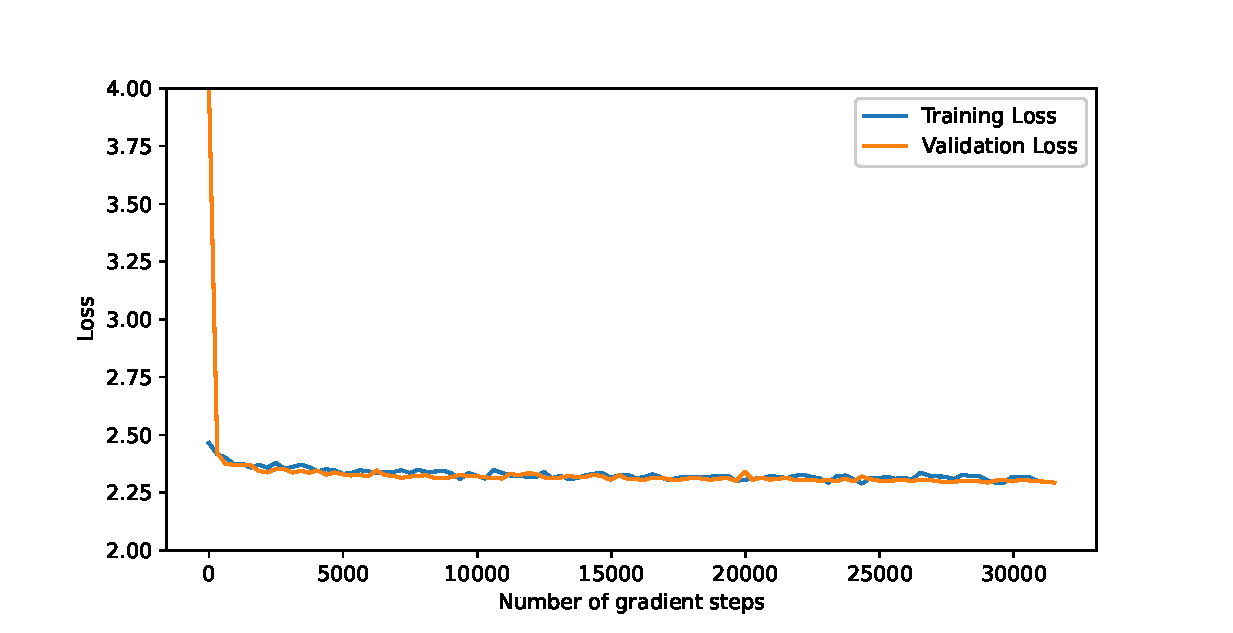
\includegraphics[width=\textwidth]{img/loss70.eps}
    \caption{Training graph for MLP3.}
    \label{fig:training}
\end{figure}


\section{Accuracy}

The top-k accuracy scores for the three \gls{MLP}s along with the benchmark accuracy for random variable selection is shown in \Cref{fig:topk}. Top k accuracy is defined as the number of selected branching variables within the top k variables as determined by the Strong Branching evaluation. 
% https://scikit-learn.org/dev/modules/model_evaluation.html#top-k-accuracy-score

MLP2 and MLP3 show near-identical accuracy, with MLP3 consistently outperformed by 2 - 3 \% at each category. Comparison with the random variable selection policy shows a considerable improvement in favor of the trained models. 

\begin{figure}
    \begin{tikzpicture}
      \begin{axis}[
        mlineplot,
        ylabel={Accuracy [\%]},
        xlabel={Top k},
        width=\textwidth,
        height=7cm,
	    ymin=0.0,   ymax=1.0,
	    xtick=data,
	    legend style={at={(0.01,0.9)},anchor=west}
      ]
        \addplot plot coordinates{(1, 0.413) (2, 0.538) (3, 0.621) (4, 0.681) (5, 0.732) (6, 0.770) (7, 0.800) (8, 0.827) (9, 0.849) (10, 0.867)};
        \addplot plot coordinates{(1, 0.437) (2, 0.568) (3, 0.653) (4, 0.717) (5, 0.767) (6, 0.805) (7, 0.835) (8, 0.860) (9, 0.881) (10, 0.899)};
        \addplot plot coordinates{(1, 0.435) (2, 0.568) (3, 0.652) (4, 0.716) (5, 0.765) (6, 0.802) (7, 0.831) (8, 0.858) (9, 0.879) (10, 0.897)};
        \addplot+ plot coordinates{(1, 0.019) (2, 0.034) (3, 0.047) (4, 0.060) (5, 0.071) (6, 0.081) (7, 0.090) (8, 0.098) (9, 0.107) (10, 0.115)};
        %\addplot+[samples=100] {sin(deg(2*x))};
        \legend{MLP1,MLP2,MLP3,Random}
        
      \end{axis}
    \end{tikzpicture}
    \caption{Top k accuracy of trained models and random variable selection on test set. MLP2 and MLP3 nearly indistinguishable.}
    \label{fig:topk}
\end{figure}
% 0 0.0 acc@1: 43.7 acc@2: 56.8 acc@3: 65.4 acc@4: 71.7 acc@5: 76.6 acc@6: 80.3 acc@7: 83.3 acc@8: 85.9 acc@9: 88.0 acc@10: 89.9

% 61 acc@0:  0.0 acc@1: 41.3 acc@2: 53.8 acc@3: 62.1 acc@4: 68.1 acc@5: 73.2 acc@6: 77.0 acc@7: 80.0 acc@8: 82.7 acc@9: 84.9 acc@10: 86.7

% 70 acc@0:  0.0 acc@1: 43.5 acc@2: 56.8 acc@3: 65.2 acc@4: 71.6 acc@5: 76.5 acc@6: 80.2 acc@7: 83.1 acc@8: 85.8 acc@9: 87.9 acc@10: 89.7


\section{Efficiency}

Five branching strategies were compared on the problem data set of three different problem sizes. The branching strategies are Full Strong Branching, Reliability Pseudo-cost branching, and the three \gls{MLP} topologies. The results are shown in \Cref{tab:results1}. \textit{Time} is the mean solution time, \textit{nodes} is the mean number of nodes in the solution graphs (calculated in accordance with the findings of Gamrath et al. \cite{gamrath2018measuring}), \textit{completed} is the number of problems where optimality was achieved within the time limit of 45 minutes and is only applicable for the large problem size. The branching strategy with the shortest mean solution time is marked bold for each problem size. 

The low-capacity MLP1 branching strategy clearly wins for small problem sizes and is slightly better for medium problem sizes. For large problem sizes, Reliability Pseudo-cost Branching is decisively better, with less than half the solution time of the \gls{MLP} strategies. 

Full Strong Branching results in solution trees orders of magnitude smaller than the \gls{MLP} counterpart. MLP1 is consistently performing faster branching than the other strategies, with respectively $8 \%, 23 \%, 48 \%$ more nodes processed than MLP2 for the three problem sizes.

\Cref{fig:barplot} shows the results for the small problem size from \Cref{tab:results1}, including $95 \%$ confidence intervals.
% \usepackage{booktabs}
 
  
\begin{scriptsize}
\begin{table}[ht]
	\centering
	\begin{tabular}{lrrrrrrr}
		\toprule
		& \multicolumn{2}{c}{Small} & \multicolumn{2}{c}{Medium} & \multicolumn{3}{c}{Large}\\ \cmidrule(lr){2-3} \cmidrule(lr){4-5} \cmidrule(lr){6-8}
		Model & Time (s) & Nodes  & Time (s) & Nodes & Time (s) & Nodes & Completed\\
		\midrule
		FSB & 5.4 &  9.7  & 135.9 &  89.4 & 2070.8 &  520.0 & 12 / 20\\
		PC &  2.5 & 378.3  &  27.3 &  3844.8 & 420.6 &  40130.6 & 20 / 20 \\
		RPC &  3.7 & 27.8  &  22.7 &  987.4 & \textbf{250.1} &  15164.4 & 20 / 20 \\
		\addlinespace
		MLP1 & \textbf{2.1} & 128.6 & \textbf{22.4} & 1224.4 & 606.4 & 22849.8 & 18 / 20\\
		MLP2 & 2.3          & 118.6 & 23.6          & 992.2 & 524.4 & 15408.4  & 18 / 20\\
		MLP3 & 3.0          & 120.2 & 51.2          & 1050.6 & 680.7 & 9889.6  & 15 / 20\\
		\bottomrule
	\end{tabular}
	\caption{Setcover.}\label{tab:results1_set}
\end{table}
\begin{table}[ht]
	\centering
	\begin{tabular}{lrrrrrrr}
		\toprule
		& \multicolumn{2}{c}{Small} & \multicolumn{2}{c}{Medium} & \multicolumn{3}{c}{Large}\\ \cmidrule(lr){2-3} \cmidrule(lr){4-5} \cmidrule(lr){6-8}
		Model & Time (s) & Nodes  & Time (s) & Nodes & Time (s) & Nodes & Completed\\
		\midrule
		FSB & 5.4 &  9.7  & 135.9 &  89.4 & 2070.8 &  520.0 & 12 / 20\\
		PC &  2.5 & 378.3  &  27.3 &  3844.8 & 420.6 &  40130.6 & 20 / 20 \\
		RPC &  3.7 & 27.8  &  22.7 &  987.4 & \textbf{250.1} &  15164.4 & 20 / 20 \\
		\addlinespace
		MLP1 & \textbf{2.1} & 128.6 & \textbf{22.4} & 1224.4 & 606.4 & 22849.8 & 18 / 20\\
		MLP2 & 2.3          & 118.6 & 23.6          & 992.2 & 524.4 & 15408.4  & 18 / 20\\
		MLP3 & 3.0          & 120.2 & 51.2          & 1050.6 & 680.7 & 9889.6  & 15 / 20\\
		\bottomrule
	\end{tabular}
	\caption{Combinatorial auction.}\label{tab:results1_cauction}
\end{table}
\begin{table}[ht]
	\centering
	\begin{tabular}{lrrrrrrr}
		\toprule
		& \multicolumn{2}{c}{Small} & \multicolumn{2}{c}{Medium} & \multicolumn{3}{c}{Large}\\ \cmidrule(lr){2-3} \cmidrule(lr){4-5} \cmidrule(lr){6-8}
		Model & Time (s) & Nodes  & Time (s) & Nodes & Time (s) & Nodes & Completed\\
		\midrule
		FSB & 5.4 &  9.7  & 135.9 &  89.4 & 2070.8 &  520.0 & 12 / 20\\
		PC &  2.5 & 378.3  &  27.3 &  3844.8 & 420.6 &  40130.6 & 20 / 20 \\
		RPC &  3.7 & 27.8  &  22.7 &  987.4 & \textbf{250.1} &  15164.4 & 20 / 20 \\
		\addlinespace
		MLP1 & \textbf{2.1} & 128.6 & \textbf{22.4} & 1224.4 & 606.4 & 22849.8 & 18 / 20\\
		MLP2 & 2.3          & 118.6 & 23.6          & 992.2 & 524.4 & 15408.4  & 18 / 20\\
		MLP3 & 3.0          & 120.2 & 51.2          & 1050.6 & 680.7 & 9889.6  & 15 / 20\\
		\bottomrule
	\end{tabular}
	\caption{Capacitated Facility Location.}\label{tab:results1_facility}
\end{table}
\begin{table}[ht]
	\centering
	\begin{tabular}{lrrrrrrr}
		\toprule
		& \multicolumn{2}{c}{Small} & \multicolumn{2}{c}{Medium} & \multicolumn{3}{c}{Large}\\ \cmidrule(lr){2-3} \cmidrule(lr){4-5} \cmidrule(lr){6-8}
		Model & Time (s) & Nodes  & Time (s) & Nodes & Time (s) & Nodes & Completed\\
		\midrule
		FSB & 5.4 &  9.7  & 135.9 &  89.4 & 2070.8 &  520.0 & 12 / 20\\
		PC &  2.5 & 378.3  &  27.3 &  3844.8 & 420.6 &  40130.6 & 20 / 20 \\
		RPC &  3.7 & 27.8  &  22.7 &  987.4 & \textbf{250.1} &  15164.4 & 20 / 20 \\
		\addlinespace
		MLP1 & \textbf{2.1} & 128.6 & \textbf{22.4} & 1224.4 & 606.4 & 22849.8 & 18 / 20\\
		MLP2 & 2.3          & 118.6 & 23.6          & 992.2 & 524.4 & 15408.4  & 18 / 20\\
		MLP3 & 3.0          & 120.2 & 51.2          & 1050.6 & 680.7 & 9889.6  & 15 / 20\\
		\bottomrule
	\end{tabular}
	\caption{Maximum Independent Set .}\label{tab:results1_indset}
\end{table}
\end{scriptsize}

\begin{figure}
    \centering
    \begin{tikzpicture}
        \begin{axis}[
          width=12cm,
          height=7cm,
          axis x line*=bottom,
          axis y line*=left,
          % nodes near coords,
          legend style={
            at={(0.5,-0.15)},
            anchor=north,
            legend columns=-1
          },
          xtick={1,2,3,4,5,6},
          xticklabels={SB,PB,RPB,MLP1,MLP2,MLP3}, 
          x tick label style={rotate=45,anchor=east},
          ymin=0,
          ymax=8,
          ybar=5pt,
          bar width=0.4cm,
          ylabel={Solution Time [\si{s}]},
          ymajorgrids=true,
          ytick={2,4,...,20}
        ]
          \addplot[color=black,fill=lightgray,error bars/.cd,
    y dir=both,y explicit] coordinates {
            (1,5.4) +- (0.0, 0.6)  %3.27)
            (2,2.5) +- (0.0, 0.24)  %1.2)
            (3,3.7) +- (0.0, 0.37) %1.9)
            (4,2.1) +- (0.0, 0.16) %0.83)
            (5,2.3) +- (0.0, 0.18) %0.93)
            (6,3.0) +- (0.0, 0.33) %1.67)
          };
        \end{axis}
  \end{tikzpicture}
  \caption{Mean solution time with 95 \% confidence intervals for small combinatorial auction problems, n = 100.}
    \label{fig:barplot}
\end{figure}
\chapter{Discussion}\label{cha:discussion}

This chapter discusses the results obtained in \Cref{cha:results} and presents ideas about further work in the field.


\section{Problem Instances}

Problem instances were only created from the class of combinatorial auctions. From the training results, it can be assumed that generating $10000$ problems is not necessary, as the model converges before all problems are seen.  

Increasing the problem size was chosen as the method for estimating the out-of-distribution efficiency of the \gls{MLP}-aided \gls{BnB}, as was done by Gupta et al. \cite{gupta2020hybrid}. Other approaches to the problem generation and generalization efficiency estimation might look into problem distributions with a temporal component, i.e. where the test samples are from a provably different distribution, without dramatically increasing the difficulty. This might be more representative of problems that are time-constrained, and will give a different estimate of the out-of-distribution generalization error.  


\section{Accuracy}

The accuracy is on par with the computationally heavy (or \gls{GPU}-dependent) Graph Convolutional Neural Network approach, with around a $3 \%$ higher accuracy than the \gls{MLP}-methods presented in \Cref{fig:topk}. MLP1 had a minor reduction in accuracy compared to MLP2 and MLP3, which had nearly indistinguishable results.   

The near-equal accuracy of the single-layer perceptron and the multi-layer perceptrons is assumed to have two possible explanations: 
\begin{enumerate}[label=(\roman*)]
    \item The training protocol is not able to discover the underlying nonlinear relation of the features to the optimal branching function. 
    \item The theoretical optimal branching function is not strongly dependent on non-linear interactions of the available features.
\end{enumerate}
The latter argument seems more likely based on the results in this project and previous experiments \cite{gupta2020hybrid} \cite{gasse2019exact}, however there are no convergence guarantees for the MLPs, and option one can therefore not be ruled out. Further analysis of the resultant linear function of MLP1 might prove further insights into this.

The fast convergence close to the optimum showed by the training graphs might indicate that a near-optimal function approximation can be found through a small amount of training data. This is consistent with the results for the three MLPs, however, this analysis was not found in Gupta et al. \cite{gupta2020hybrid}.

The practically insignificant accuracy of MLP1 and MLP2 has similar arguments. This indicates that increasing the capacity of the model is not a productive strategy for learning to branch with the current feature set. 

\section{Efficiency}

The central problem in \textit{learning-to-branch} is the trade-off between computational efficiency and the number of nodes processed. The results in \Cref{tab:results1_cauction} show that an increase in complexity can very negatively impact the solution time. MLP3 has a considerably longer solution time than MLP2, even though the average  number of evaluated nodes is only 1 \% more for MLP3. This indicates a large amount of the solution time is spent in the forward pass of the MLP. MLP1 gains a 17 \% decrease in computation time at the cost of 8 \% more nodes evaluated. The \gls{MLP} with optimal efficiency can be a higher capacity network than MLP1, however, the reduced implementation complexity of the linear model might make up for this discrepancy in accuracy. 

%Gupta et al. \cite{gupta2020hybrid} recommends the \gls{FiLM} model for an efficient forward pass, however, the results in this project show that linear models can give close to the same accuracy, and would therefore be preferred over more complex models when the accuracy discrepancy remains small.  


\section{Further Work}

The time-consuming process of further verification of the \gls{MLP} models on more problem sets and averaging over random seeds as in Gupta et al. \cite{gupta2020hybrid} remains to be done to increase the certainty of the findings. After this, a comprehensive cross-check of the results in the two studies might lead to valuable insights into the differences in the approaches.   

Further work in the field should also strive to compare results with the top commercial solvers IBM CPLEX and Gurobi \cite{anand2017comparative}. The automatic tuning of the highly parameterized commercial optimization solvers has also been shown to yield significant improvements in solution time \cite{hutter2010automated}, and is therefore advised to include in further and more comprehensive comparisons.  

The results in this project show that for the features of the branching variables, a linear classifier might suffice to outperform Reliability Pseudo-cost Branching as compared to more demanding methods. It seems reasonable to assume that there can be a significant increase in efficiency with an implementation of the linear branching rule, either directly into \gls{SCIP} or via a more performance-conscious interface with PySCIPOpt. The assumed improvement in efficiency might further encourage work on learned function approximations as components of solution algorithms. Another opportunity with linear classifiers showing close-to-optimal accuracy with Deep Neural Networks is the increase in methods for parameter analysis from the resulting optimal model. Analyzing this can yield useful insights into the core components of the successful functions, which appears unexplored in the literature.

The work in this field remains on artificial problems, however, there would be great interest in a practical implementation on real-world optimization problems, e.g. an optimal traffic routing algorithm running on an embedded system. 

What appears unexplored by the community working on supervised learning in \gls{BnB} is the regression problem of predicting the Strong Branching score, as this is an unused feature. The correlation of the variable features and the objective function improvement might further provide insights into the possibilities and limitations of function approximations to variable selection algorithms. 

A recurring approach mentioned in the context of improving \gls{BnB} is the Reinforcement Learning approach. This appears to be under development, with results in review by Etheve et al. \cite{etheve2020reinforcement} and development of a training suite by Prouvost et al. \cite{prouvost2020ecole}. On a larger scale, the work on learning-to-branch fits in the larger context of learned algorithms replacing expert-created algorithms. This has the potential to eventually remove the human component to algorithm construction. For now, closer attention to the features and correlations of the variable scoring might be the more fruitful endeavor, as the results in this project show that the deep learning approach does not yield significantly better results. 


\section{Research Questions}

Now, we return to the research questions presented in \Cref{sec:questions}:
\begin{enumerate}[label=(\roman*)]
    \item \textit{Can Multi-Layer Perceptrons decrease the running time of Branch and Bound running on the \Gls{CPU}?}
\end{enumerate}
Based on the results presented in \Cref{cha:results}, the conclusion is \textit{yes} when compared to the Full Strong Branching, Pseudo-cost Branching and Reliability Pseudo-cost Branching strategies found in the SCIP Optimization solver. 
\begin{enumerate}[resume*]
    \item \textit{What is the impact of different \gls{MLP} model sizes on the accuracy and efficiency of the Branch and Bound algorithm}?
\end{enumerate}
Both accuracy and efficiency was found to vary over the different \gls{MLP} design choices. This implies that larger models, at least up to a point, would see higher accuracy in branching variable choice. However, increased model complexity gives slower inference time, showing that for the conducted experiments, the best performing model was a linear model.
\begin{enumerate}[resume*]
    \item \textit{Are there more research opportunities for \gls{MLP}s in Branch and Bound?}
\end{enumerate}
Positive results indicate many opportunities in this research field. Firstly, further verifying the results in this project on other problems and configurations is needed for a larger degree of certainty on their usefulness. Further, the analysis of the \gls{MLP}s might give the insights mentioned in \cite{lodi2017learning}, that are still unanswered, particularly the single-layer model is a good candidate for this.   
\chapter{Conclusion}\label{cha:conclusion}

The experiments show that Multi-Layer Perceptrons can improve the running time of \gls{BnB} over the default method in the SCIP Optimization solver running purely on the CPU. Three \gls{MLP}s of varying capacity and computational complexity were tested for variable choice accuracy and efficiency when integrated into the SCIP solver. The two higher-capacity models showed identical accuracy, but the computational complexity of the largest \gls{MLP} was too high to result in an improved running time of the algorithm on the test problems. MLP1, the best-performing method, was a model with no hidden layers and is therefore identical to a linear model. 



Increasing the model capacity showed no accuracy increase, and is shown to increase computation time notably. This proves the importance of model selection with minimal computational complexity, at the expense of some accuracy. Implementations of purely linear methods will be simpler to do directly in the solver. It can be assumed that the overhead of working via the PySCIPOpt interface and performing the computations in a PyTorch-compliant manner negatively impacts efficiency. The possibilities for implementing the learned branching strategies in the most computationally efficient way should be evaluated, as this might greatly improve the results for all machine learning aided \gls{BnB}.  

Firstly, for the conducted experiments in this project: Fewer problem sets, fewer experiments, and no accounting for the impact of randomized seeds was performed in this project, as compared to the works by Gasse et al. \cite{gasse2019exact} and Gupta et al. \cite{gupta2020hybrid}. These experiments are time-consuming, however for a higher degree of certainty in the validity of the results, this might be necessary to explore in future work. The initiative to standardize comparisons of learned branching strategies will be productive for the research community, however, the current standards imply multiple weeks of running experiments for researchers with only one computer available, which is the reason for the reduced number of experiments in this project.   

The results indicate a possible shift away from the deep learning approach, given the features currently available. Deep learning based models are unlikely to be outcompeted on accuracy, however, good linear models indicate great opportunities for analyzable, tractable, classical methods that are faster to implement. Researchers are encouraged to explore these methods and analyze the nature of the currently used feature set developed by Khalil \cite{khalil2020towards} and Gupta et al. \cite{gupta2020hybrid}.

In conclusion, the results for using Multi-Layer Perceptrons in learning to branch are very positive. Experiments indicate that linear models might be equally suited as deep networks. Accurate linear methods can provide opportunities for evaluating the current feature-set used by the researchers in the field and is assumed to be a fertile area of research which is probable to gain community attention and new insight.    

%\begin{chapquote}{Thomas Aquinas, \textit{Summa Theologica}}
%``Quod potest compleri per pauciora principia, non fit per plura.\footnote{It is superfluous %to suppose that what can be accounted for by a few principles has been produced by many.}''
%\end{chapquote}

% Diskusjonskapittel
% Rød tråd: Accuracy vs. efficiency
%\input{tex/log}
%%\appendix
%%%!TEX root = ../Thesis.tex
\chapter{Appendix}\label{cha:appendix-my-appendix}
%

\section{Time and Node Distributions}\label{sec:distributions}
\begin{figure}[h]
    \centering
    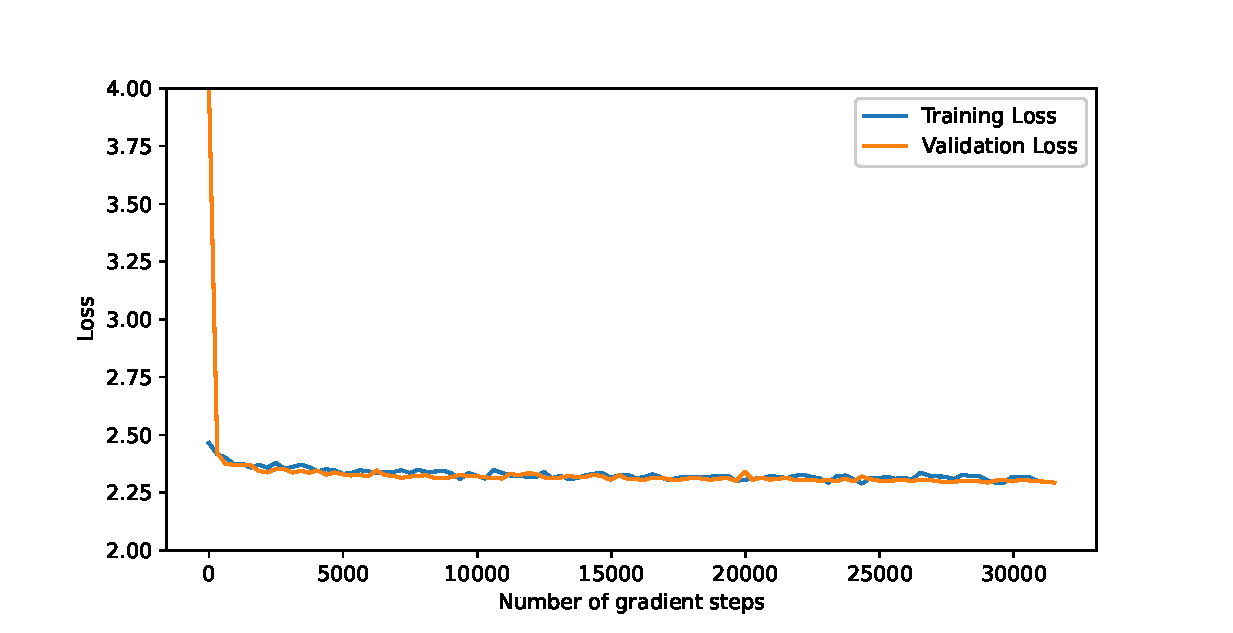
\includegraphics[width=\textwidth]{img/loss70.eps}
    \caption{Histogram of nodes for pseudo cost branching and MLP2.}
    \label{fig:node_histogram}
\end{figure}


\section{Linear Model Coefficients}\label{sec:coefficients}
...


\backmatter
\printbibliography[heading=bibintoc,title={References}]

\end{document}
